\documentclass{article}

\usepackage[letterpaper,margin=1in]{geometry}
\usepackage{graphicx} % Required for inserting images
\usepackage{amsmath}
\usepackage{amsthm}
\usepackage{amssymb}
\usepackage{booktabs}
\usepackage{longtable,pdflscape}
\usepackage{multirow}
\usepackage{mathrsfs}
\usepackage{makecell}
\usepackage{array}
\usepackage{caption}
\usepackage[authoryear,round,sort]{natbib}
\usepackage{hyperref}
\usepackage{xurl}
\usepackage{authblk}

\usepackage{placeins}
\usepackage{float}

\usepackage{relsize}              % in your preamble
\newcommand{\bigveebar}{%
  \mathop{\mathlarger{\mathlarger{\veebar}}}\displaylimits%
}
\newtheorem{proposition}{Proposition}[section]
\newtheorem{theorem}{Theorem}[section]
\newtheorem{corollary}{Corollary}[section]

% Commands used to include orcid (taken from https://gugushvili.github.io/blog/2019/08/09/orcid)
\usepackage{tikz}
\definecolor{lime}{HTML}{A6CE39}
\DeclareRobustCommand{\orcidicon}{
	
\begin{tikzpicture}
	\draw[lime, fill=lime] (0,0)
	circle [radius=0.16]
	node[white] {{\fontfamily{qag}\selectfont \tiny ID}};
	\draw[white, fill=white] (-0.0625,0.095)
	circle [radius=0.007];
	\end{tikzpicture}
	\hspace{-2mm}
}
\foreach \x in {A, ..., Z}{\expandafter\xdef\csname orcid\x\endcsname{\noexpand\href{https://orcid.org/\csname orcidauthor\x\endcsname}
			{\noexpand\orcidicon}}
}
\newcommand{\orcidauthorA}{0000-0002-8308-5016} % For David Bernal
\newcommand{\orcidauthorB}{0000-0002-4474-3266} % For Albert Lee
\newcommand{\orcidauthorC}{0009-0003-8823-8055} % For Woosik Kim

\newcommand{\david}[1]{\textcolor{red}{D: #1}}
\newcommand{\albert}[1]{\textcolor{blue}{A: #1}}

\title{Black-Box Configuration Search for Generalized Disjunctive Programming}
\author[1]{Albert Joon Lee\orcidB}
\author[2]{Woosik Kim\orcidC}
\author[1,*]{David E. Bernal Neira\orcidA}

\affil[1]{Davidson School of Chemical Engineering, Purdue University, West Lafayette, IN 47907, USA}
\affil[2]{Elmore Family School of Electrical and Computer Engineering, Purdue University, West Lafayette, IN 47907, USA}

\date{*Email: dbernaln@purdue.edu}

\setlength{\emergencystretch}{2em}
\begin{document}

\maketitle

\begin{abstract}
Selecting configurations in generalized disjunctive programming (GDP) can require repeated, costly subproblem evaluations.
Existing external integer representations allow these logical choices to be explored by derivative-free search.
We ask whether alternative black-box search methods reach reference targets more often than budget-limited discrete steepest descent under common initial configurations and evaluation budgets.
Tests cover 21 Grid problems and four process GDP families, comparing RBFOpt, Branch-and-Model (BAM), factorization-machine-based optimization with simulated annealing (FMQA-SA), and sampling controls.
Completion costs are estimated from recorded searches using stored objective responses and separately measured subproblem costs.
Here we show that alternative search methods can improve target-hit rates, but the gains depend on the problem and evaluation budget.
RBFOpt reaches the target in 45 of 60 continuous stirred-tank reactor (CSTR) runs versus 14 for discrete steepest descent; on the dynamic benchmark, it reaches all ten targets at an evaluation budget of \(B=12\), while discrete steepest descent first does so at \(B=30\).
On Grid at an evaluation budget of \(B=100\), RBFOpt reaches the target in 81.4\% of runs, compared with 48.1\% for discrete steepest descent, 70.0\% for BAM, and 21.4\% for uniform sampling.
BAM leads at the smallest Grid budget through initial sampling, whereas discrete steepest descent reaches more targets on Column and Small Batch.
These results support black-box optimization on existing external integer representations as an option for GDP configuration search.
Higher target-hit rates do not necessarily reduce total computational cost, so both measures should guide method selection.
% \david{Let's rewrite the abstract using https://imgv2-2-f.scribdassets.com/img/document/277786588/original/2a6edb71c4/1?v=1}
\end{abstract}

\noindent\textbf{Keywords:} Generalized disjunctive programming; Black-box optimization; Derivative-free optimization; Surrogate modeling; Process systems engineering; Computational benchmarking.

\section{Introduction}
In chemical process design, evaluating a single candidate configuration can require costly optimization or simulation, making the choice of which configuration to explore next a central computational challenge.
Process design involves discrete decisions, such as equipment selection, the number of processing stages, and operating modes, along with continuous variables such as flow rates, temperatures, and equipment sizes.
Generalized disjunctive programming (GDP) provides a framework to represent these decisions through Boolean variables, logical propositions, and conditional constraints~\citep{raman1994modelling}.
In logic-based GDP solution methods, fixing the Boolean variables associated with a selected configuration determines which constraints remain active and yields a reduced optimization subproblem.
When all discrete decisions are fixed, this subproblem can be formulated as a nonlinear programming (NLP) problem.
Exploring multiple configurations may therefore require repeatedly solving NLP subproblems, which can be computationally expensive.
Consequently, identifying high-quality configurations with fewer evaluations of NLP subproblems is an important objective in solving GDP problems.

Conventional GDP solution methods generally rely on mixed-integer nonlinear programming (MINLP) reformulations or logic-based decomposition.
The Big-\(M\) and Hull reformulations transform disjunctive constraints into algebraic formulations~\citep{raman1994modelling,grossmann2003hull}, while logic-based approaches select discrete configurations and solve the corresponding reduced subproblems~\citep{turkay1996logic,bergamini2005logic}.
In logic-based approaches, the strategy used to select discrete configurations can significantly affect the number of subproblem evaluations required.

Discrete-Steepest Descent (D-SDA) was previously applied to process superstructure optimization by \citet{linan2020optimal}.
Building on this approach, our previous work introduced the Logic-Based Discrete-Steepest Descent (LD-SDA), which represents ordered Boolean decisions using external integer variables~\citep{ovalle2025logic}.
LD-SDA explores the resulting integer space through neighborhood search and discrete line search, evaluating selected configurations by solving their corresponding reduced optimization subproblems.
However, as a local search method, LD-SDA may converge to different locally optimal solutions depending on the starting point and the selected neighborhood~\citep{peng2024dynamic}.

We use the existing external integer representation to search GDP configurations with black-box optimization methods.
Surrogate-based derivative-free optimization (DFO) uses accumulated objective observations to guide new evaluations~\citep{larson2019derivative}.
RBFOpt builds radial basis function surrogates and balances predicted objective values with exploration~\citep{costa2018rbfopt}.
The comparison includes Branch-and-Model (BAM)~\citep{ma2023bam} and a variant of the factorization machine with quantum annealing (FMQA) framework~\citep{kitai2020designing}.
We use classical simulated annealing in place of quantum annealing and denote this variant FMQA-SA.
We ask whether these methods reach reference targets more often than budget-limited D-SDA under common initial configurations and limited evaluation budgets.
Uniform sampling provides a baseline without objective-dependent candidate selection.

Fewer evaluations do not necessarily imply lower computational cost, because evaluation costs vary and candidate selection incurs overhead~\citep{more2009benchmarking}.
We therefore compare how often each method reaches the target, along with configuration-evaluation costs and search overhead.
The methods share precomputed configuration responses, while response handling and stopping remain implementation-specific.
The contributions are as follows:
\begin{itemize}
\item A comparison of black-box configuration search methods on the existing GDP external integer representation using 21 Grid-GDP benchmarks and four published process GDP families, with common initial configurations, evaluation budgets, and reference targets.
\item An analysis of how performance varies across problems and evaluation budgets, distinguishing target-reaching rates, configuration-evaluation costs, and search overhead.
\end{itemize}

\section{Background}

\subsection{Generalized Disjunctive Programming and Fixed-Configuration Evaluation}

GDP represents operational and design alternatives using Boolean variables and associated algebraic constraints~\citep{raman1994modelling}.
The original continuous variables have domain \(\mathcal X=[\underline{\mathbf x},\overline{\mathbf x}]\subseteq\mathbb R^{n_x}\).
The original integer variables have domain \(\mathcal Z=[\underline{\mathbf z},\overline{\mathbf z}]\cap\mathbb Z^{n_z}\).
Let \(K\) index the disjunctions and \(D_k\) index the disjuncts in disjunction \(k\in K\).
Each disjunct \(i\in D_k\) has a Boolean variable \(Y_{ik}\).
The GDP formulation is given by
\begin{equation}\label{eqn:gdp.general}
\begin{aligned}
\min_{\mathbf x,\mathbf z,\mathbf Y}\quad & f(\mathbf x,\mathbf z)\\
\text{s.t.}\quad &\mathbf g(\mathbf x,\mathbf z)\leq\mathbf 0,\\
&\bigveebar_{i\in D_k}\left[
\begin{gathered}
Y_{ik}\\
\mathbf h_{ik}(\mathbf x,\mathbf z)\leq\mathbf 0
\end{gathered}\right],\qquad k\in K,\\
&\Omega(\mathbf Y)=\mathrm{True},\\
&\mathbf x\in\mathcal X,\quad\mathbf z\in\mathcal Z,\quad
\mathbf Y\in\{\mathrm{False},\mathrm{True}\}^{n_y}.
\end{aligned}\tag{GDP}
\end{equation}
Here, \(f\) is the objective function, \(\mathbf g\) represents the global constraints, and \(\mathbf h_{ik}\) represents the constraints associated with each disjunct.
The operator \(\veebar\) requires that exactly one disjunct be selected within each disjunction.
Logical propositions \(\Omega(\mathbf Y)\) impose additional relationships between Boolean variables.

Following the external-variable reformulation of \citet{ovalle2025logic}, each ordered group of \(m_j\) Boolean alternatives is represented by an external integer variable \(\xi_j\in\{1,\ldots,m_j\}\), which identifies the selected alternative.
Let \(n_E\) denote the number of external integer variables, and \(\mathcal Y_{\mathrm{logic}}\) the set of Boolean assignments that satisfy the conditions \texttt{exactly-one}, and \(\Omega(\mathbf Y)\).
The external-variable lattice and its logically admissible subset are
\begin{equation}\label{eqn:external.lattice}
\begin{aligned}
\mathcal L_E&=\prod_{j=1}^{n_E}\{1,\ldots,m_j\},\\
\mathcal E_{\mathrm{adm}}&=\{\boldsymbol\xi\in\mathcal L_E:
\mathbf Y(\boldsymbol\xi)\in\mathcal Y_{\mathrm{logic}}\}.
\end{aligned}
\end{equation}
For each logically admissible configuration \(\boldsymbol\xi\), the corresponding Boolean variables are fixed, yielding the following reduced optimization subproblem:

\begin{equation}\label{eqn:Sub}
\begin{aligned}
\Phi(\boldsymbol\xi)=\inf_{\mathbf x,\mathbf z}\quad &f(\mathbf x,\mathbf z)\\
\text{s.t.}\quad &\mathbf g(\mathbf x,\mathbf z)\leq\mathbf 0,\\
&\mathbf h_{ik}(\mathbf x,\mathbf z)\leq\mathbf 0
\quad\text{for all }(i,k)\text{ with }Y_{ik}(\boldsymbol\xi)=\mathrm{True},\\
&\mathbf x\in\mathcal X,\quad\mathbf z\in\mathcal Z.
\end{aligned}\tag{Sub}
\end{equation}
Here, \(\Phi(\boldsymbol\xi)\) represents the optimal objective value of the reduced subproblem.
The reduced subproblem is an NLP when all remaining decision variables are continuous.
If the reduced subproblem is infeasible, we define \(\Phi(\boldsymbol\xi)=+\infty\).

When the external-variable mapping represents all logically admissible Boolean configurations, the original GDP can be expressed as the following upper-level optimization problem~\citep{ovalle2025logic}:
\begin{equation}\label{eqn:outer.value}
\min_{\boldsymbol\xi\in\mathcal E_{\mathrm{adm}}}\Phi(\boldsymbol\xi).
\end{equation}
A logically admissible configuration may still yield an infeasible reduced subproblem.

\subsection{Conventional GDP Solution Approaches}

Big-\(M\) and Hull reformulations transform GDP models into mixed-integer nonlinear programming (MINLP) formulations by associating Boolean variables \(Y_{ik}\) with binary variables \(y_{ik}\) and translating logical propositions into algebraic constraints~\citep{raman1994modelling,grossmann2003hull}.
In the Big-\(M\) reformulation, the disjunctive constraints are expressed as \(\mathbf h_{ik}(\mathbf x,\mathbf z)\leq\mathbf M_{ik}(1-y_{ik})\), where the inequality is applied componentwise.
The Big-\(M\) values must be sufficiently large to render the corresponding constraints redundant when \(y_{ik}=0\), but excessively large values can weaken the continuous relaxation and cause numerical difficulties.

Hull reformulations introduce disaggregated variables, linking constraints, and bounds scaled by binary indicators~\citep{grossmann2003hull}.
Disjunctive constraints are imposed on the disaggregated variables when \(y_{ik}=1\), while \(y_{ik}=0\) forces these variables to zero, making the corresponding disjunct inactive.
For convex disjunctive sets, this formulation can provide a stronger continuous relaxation than Big-\(M\), although it introduces additional variables and constraints.
For nonconvex GDP problems, the Hull reformulation does not guarantee a convex reformulated model or global optimality~\citep{chen2022pyomogdp}.

% \david{There is a missing paragraph here saying that logic-based methods apply to the GDP directly}
Logic-based methods address GDP problems directly by exploiting their logical and disjunctive structure to select discrete configurations and construct the corresponding optimization subproblems.
Logic-based outer approximation (LOA) alternates between a mixed-integer master problem and fixed-configuration NLP subproblems~\citep{turkay1996logic}.
Under suitable convexity and regularity assumptions, the master problem uses linearization cuts to obtain lower bounds, while feasible solutions to the NLP subproblem provide upper bounds.
For nonconvex GDP problems, these linearizations may not provide valid global lower bounds, motivating global logic-based outer approximation (GLOA), which requires globally valid relaxations and subproblem bounds.
\citet{bergamini2005logic} developed a GLOA approach for process networks using piecewise under- and overestimators.

GDPopt provides implementations of logic-based methods within Pyomo.GDP~\citep{chen2022pyomogdp,pyomoGDPopt}.
Its relaxation with integer cuts (RIC) method uses a mixed-integer linear programming (MILP) relaxation to select configurations and adds no-good cuts to exclude evaluated discrete assignments, without generating the successive outer-approximation cuts used by LOA~\citep{pyomoGDPopt}.

LD-SDA is an existing alternative that searches ordered external configurations by improving neighborhood moves and discrete line searches~\citep{ovalle2025logic}.
It selects the best improving neighbor, continues along the resulting direction while improvement persists, and resumes neighborhood exploration.
The present work uses this discrete-search structure as a reference and compares other configuration-selection strategies and their computational costs.

\subsection{Derivative-Free Optimization Solvers}

Derivative-free optimization (DFO) uses function observations without requiring derivatives of the objective with respect to the search variables~\citep{larson2019derivative}.
Black-box configuration search selects configurations using their evaluation responses without accessing the subproblem equations.
For GDP configuration search, the outer method can be derivative-free, even if its evaluation routine uses a derivative-based nonlinear solver.
D-SDA also uses this derivative-free interface, although it does not construct a surrogate model.
% \david{Missing sentence(s) explaining how this is a logic-based method: the upper model optimizes over the space of reformulated external variables and can provide extra constraints, some of which are encoded in the external-variable reformulation.}
The upper-level search operates over external integer variables that represent the logical decisions in the GDP. 
Some logical restrictions are embedded in the external-variable reformulation, while additional constraints can be imposed on the configuration space.
% \david{There is a sudden jump to surrogate methods here. You need a connecting sentence before}
One approach to DFO uses surrogate models to guide the search.
Surrogate methods seek to reduce expensive evaluations by fitting models to observed data, with computational cost arising from both objective evaluations and model-based candidate selection.

\subsubsection{Branch-and-Model (BAM)}
Branch-and-Model (BAM) combines domain partitioning with local surrogate construction~\citep{ma2023bam}.
The evaluated points define boxes, and a potentially optimal selection procedure identifies regions for further modeling and search.
Within selected boxes, Automated Learning of Algebraic Models (ALAMO) constructs sparse algebraic models from nearby observations~\citep{cozad2014learning}.
BARON optimizes these local models to propose candidates, while box-size exploration maintains broader coverage~\citep{ma2023bam,bamManual,sahinidis1996baron}.
Thus, BARON acts on learned surrogates within BAM; it is not solving the original GDP through this interface.
Its support for integer restrictions allows for the configuration domains considered here~\citep{bamManual}.

\subsubsection{Factorization-Machine-Based Optimization}

A second-order factorization machine (FM) models individual feature effects and pairwise interactions through shared latent parameters~\citep{rendle2010factorization}.
For a binary encoding \(\mathbf b\in\{0,1\}^{m}\) of an external integer configuration \(\boldsymbol\xi\), the FM fit surrogate is
\begin{equation}\label{eqn:fm.surrogate}
\widehat\Phi_{\mathrm{FM}}(\mathbf b)
=\beta_0+\sum_{i=1}^{m}\beta_i b_i
+\sum_{i=1}^{m-1}\sum_{j=i+1}^{m}
\langle\mathbf a_i,\mathbf a_j\rangle b_i b_j,
\end{equation}
where \(\widehat\Phi_{\mathrm{FM}}(\mathbf b)\) denotes the predicted training response, \(m\) is the number of binary features, \(\beta_0\) is the intercept, \(\beta_i\) is the linear coefficient of \(b_i\), and \(\mathbf a_i\in\mathbb R^r\) is its latent vector of dimension \(r\).
The inner product \(\langle\mathbf a_i,\mathbf a_j\rangle\) determines the pairwise interaction coefficient.
The model parameters are learned from the evaluated configurations and their corresponding training responses.

For binary inputs, \(b_i^2=b_i\), the fitted model is a binary quadratic model.
 % \david{I don't know if dropping is the right verb here as we still record it for correcting the terms} 
Excluding the constant term \(\beta_0\) gives the following quadratic unconstrained binary optimization (QUBO) problem:
\begin{equation}\label{eqn:fm.qubo}
\min_{\mathbf b\in\{0,1\}^{m}}\mathbf b^{\mathsf T}\mathbf Q\mathbf b,
\qquad
Q_{ij}=\begin{cases}
\beta_i,&i=j,\\
\langle\mathbf a_i,\mathbf a_j\rangle,&i<j,\\
0,&i>j.
\end{cases}
\end{equation}
The QUBO describes the learned surrogate, not an exact algebraic reformulation of the GDP.
Moreover, a binary string need not decode to a logically admissible configuration in the domain.

The factorization machine with quantum annealing (FMQA) framework combines FM surrogate fitting with annealing-based candidate generation~\citep{kitai2020designing}.
Based on observed evaluations, the method fits the FM, samples binary candidates from the resulting quadratic model, and evaluates a selected decoded configuration through the objective-evaluation routine before updating the training data.

The FMQA simulated annealing variant (FMQA-SA) uses classical simulated annealing to sample binary candidates from the learned QUBO.
Temperature-dependent acceptance of uphill moves supports exploration, while gradual cooling favors lower-energy solutions~\citep{kirkpatrick1983optimization}.
In this study, no quantum hardware was used.

\subsubsection{RBFOpt}
RBFOpt is an open-source surrogate optimizer for bounded black-box problems, with support for continuous, integer, and categorical variables~\citep{costa2018rbfopt,nannicini2021implementation}.
Given \(N\) observed objective values in external integer configurations \(\boldsymbol\xi^{(1)},\ldots,\boldsymbol\xi^{(N)}\), RBFOpt constructs a radial basis function (RBF) surrogate model of the form
\begin{equation}\label{eqn:rbf.surrogate}
\widehat\Phi_N(\boldsymbol\xi)
=\sum_{r=1}^{N}\lambda_r\varphi\!\left(\|\boldsymbol\xi-\boldsymbol\xi^{(r)}\|_2\right)
+p(\boldsymbol\xi),
\end{equation}
where \(\widehat\Phi_N(\boldsymbol\xi)\) approximates the objective value for a candidate configuration \(\boldsymbol\xi\), \(\lambda_r\) are interpolation coefficients determined from the observed values, \(\varphi\) is the RBF kernel evaluated at the Euclidean distance between configurations, and \(p(\boldsymbol\xi)\) is a polynomial tail depending on the selected kernel.

Candidate selection balances low predicted values against exploration away from evaluated points.
The metric stochastic response surface method (MSRSM) combines scaled surrogate predictions and distances to existing samples, changing their relative weights during the search~\citep{regis2007stochastic}.
New objective evaluations update the model.

\section{Experimental Methods}
\label{sec:methodology}\label{sec:cases}

\subsection{Benchmark problems: Grid-GDP}
\label{sec:grid-gdp-formulation}
We consider 21 two-dimensional test functions adapted from the Quantum Hamiltonian Descent benchmark collection~\citep{qhdBenchmarks}.
Each is sampled at 31 equally spaced values per coordinate, giving 961 configurations.
For each benchmark function, let \([\ell_x,u_x]\) and \([\ell_y,u_y]\) denote the coordinate bounds, and let \(I=J=\{0,\ldots,30\}\) be the corresponding index sets.
The Grid optimizers receive \((i,j)\in\{0,\ldots,30\}^{2}\) directly.
Relative to the one-based convention in Section~2.1, \((\xi_1,\xi_2)=(i+1,j+1)\) is only a relabeling of alternatives.
\texttt{FMQA-SA} encodes each Grid index in five unsigned bits and rejects decoded values of 31.
The physical coordinates are defined as
\begin{equation}\label{eqn:grid-coordinates}
a_i=\ell_x+\frac{i(u_x-\ell_x)}{30},\qquad
b_j=\ell_y+\frac{j(u_y-\ell_y)}{30}.
\end{equation}

Let \(f\) denote the original analytical objective function and let \(L\) and \(U\) be its minimum and maximum over the \(31\times31\) lattice.
Both constants are obtained by exhaustive preprocessing of all 961 lattice points prior to any search.
A normalized target tolerance of \(10^{-5}\) corresponds to \(10^{-5}(U-L)\) in raw objective units, so equal normalized tolerances do not need to define equally large target sets.
Supplementary Table~\ref{tab:grid-domains} gives target-set sizes for all functions.
Full-precision normalization constants are available in the repository (Supplementary Section~\ref{sec:supp-data}).
Each benchmark function is represented by the following GDP:
\begin{equation}\label{eqn:grid-gdp}
\begin{aligned}
\min_{x,y,Y^x,Y^y}\quad & F(x,y)=\frac{f(x,y)-L}{U-L}\\
\mathrm{s.t.}\quad &
\bigvee_{i\in I}\left[\begin{array}{c}Y_i^x\\x=a_i\end{array}\right],\qquad
\bigvee_{j\in J}\left[\begin{array}{c}Y_j^y\\y=b_j\end{array}\right],\\
&\operatorname{ExactlyOne}(Y_0^x,\ldots,Y_{30}^x),\\
&\operatorname{ExactlyOne}(Y_0^y,\ldots,Y_{30}^y),\\
&\ell_x\leq x\leq u_x,\qquad \ell_y\leq y\leq u_y,\\
&Y_i^x,Y_j^y\in\{\mathrm{False},\mathrm{True}\}.
\end{aligned}
\end{equation}
The two exclusive disjunctions contain 62 coordinate-selection Boolean indicators.
The objective retains the explicit mathematical expression.
Consequently, the conventional GDP methods receive the expression and its disjunctive structure, whereas the DFO methods observe only objective values returned at their selected coordinates.

Fixing both coordinate disjunctions fixes \(x\) and \(y\), leaving no remaining original continuous degrees of freedom.
Thus, the measured fixed-point \texttt{IPOPT}~\citep{wachter2006implementation} evaluations characterize fresh model preparation, solver invocation, and verification, rather than a difficult continuous optimization subproblem.
The unfixed objective functions remain nonlinear and generally nonconvex, so Big-\(M\) and Hull produce MINLP representations.
The complete mathematical definitions and coordinate domains of the 21 benchmark functions are provided in Supplementary Sections~\ref{sec:supp-domains}-\ref{sec:supp-objectives} (Table~\ref{tab:grid-domains})~\citep{rbfoptTestArchive,qhdBenchmarks}.

\subsection{Process GDP benchmark problems}
\label{sec:process-cases}
The process benchmarks include a CSTR network~\citep{linan2020optimal}, a 17-stage distillation column~\citep{ghouse2018comparative}, and a small batch plant~\citep{kocis1988global}.
We use their GDP formulations reported by \citet{ovalle2025logic}, and the nine-stage nonlinear mode-switching model of \citet{peng2024dynamic}.
% \david{This is the citation of the GDP reformulation of the problems, but above add the citation of the original problems}
Their objectives minimize the total reactor volume (\texttt{CSTR}), condenser and reboiler duties, plus the active tray cost (\texttt{Column}), the investment cost (\texttt{Small Batch}), and the negative integral of the squared state (\texttt{Dynamic}).
The external variables represent the reactor/feed cutoff and recycle location (\texttt{CSTR}), reflux and boilup positions (\texttt{Column}), parallel unit counts (\texttt{Small Batch}), and final stages of modes 1 and 2 (\texttt{Dynamic}).
For these process benchmarks, fixing the external choices leaves only continuous variables, so the resulting subproblems are NLPs.
The \texttt{CSTR} superstructure contains \(N\) potential reactor positions, where \(N\in\{5,10,15,20,25,30\}\).
We denote each \texttt{CSTR} instance by its size parameter \(N\), such as \texttt{CSTR30} for \(N=30\).
\texttt{Dynamic} uses 30 finite elements per stage and three Radau collocation points.
The reference configurations in external variable coordinates are \((N,N)\) for \texttt{CSTR}, \((13,4)\) for \texttt{Column} (physical trays \((14,5)\)), \((2,2,1)\) for \texttt{Small Batch}, and \((1,4)\) for \texttt{Dynamic}.
The full GDP formulations of the \texttt{CSTR}, \texttt{Column}, and \texttt{Small Batch} benchmarks are provided in Appendices A.1-A.3 of \citet{ovalle2025logic}, respectively, while the \texttt{Dynamic} formulation is described in Section IV.C of \citet{peng2024dynamic}.
External-variable mappings for the three design cases are provided in Appendices B.1, B.2, and B.4 of \citet{ovalle2025logic}.
% \david{At least say the section (I believe it was the appendices of the paper with Ovalle)}.
The \texttt{CSTR} volume is reported in liters and the \texttt{Small Batch} investment in the source model's dollars.
The \texttt{Column} uses the source model's weighted cost proxy based on duties and active trays.
The model sizes and unit conventions are given in the Supplementary Section~\ref{sec:supp-models} (Table~\ref{tab:supp-model-sizes}).
\texttt{Dynamic} is an abstract benchmark with no calibrated physical units for state or time.
Minimizing its negative squared-state integral favors greater integrated state magnitude and tests mode sequencing coupled to dynamic equations.

% \david{What is meant by coverage?}
Table~\ref{tab:process-cases} summarizes the original GDP and DFO candidate domains, the number of configurations with \texttt{IPOPT}-accepted objective values, the number of configurations with measured evaluation times, and the evaluation budgets.
The process searches use frozen objective tables from fixed-configuration \texttt{IPOPT} evaluations; only accepted finite objectives are used as valid lookup objectives.
The objective, acceptance status, and point cost are taken from the same recorded evaluation attempt for the same model, CSTR size, and external-variable tuple.
Measured coverage includes all configurations in each DFO candidate box, including unsuccessful and structural-rejection evaluations.
The evaluation budget \(B\) limits the total number of objective evaluations, including initialization, repeated calls, and unsuccessful evaluations.
The full GDP box precedes the logical and algebraic feasibility restrictions.
\texttt{Column} searches \(\{8,\ldots,15\}\times\{1,\ldots,8\}\) (64 coordinates), the logical domain of its original \(\{1,\ldots,15\}^{2}\) box.
Other cases use their full boxes.
The \texttt{Column} bounds encode the reflux and boilup placement restrictions; algebraic constraints are still checked during configuration evaluation.
All DFO methods use this box, and the \texttt{Column} conclusions apply only to it.
For \texttt{CSTR}, recycle/feed ordering admits \(N(N+1)/2\) logical candidates, but not all yield objective values satisfying the solver acceptance criteria defined in Section~\ref{sec:protocol}.
% \david{What is meant by an accepted solution?}
The \texttt{CSTR} comparisons do not isolate scalability: evaluation budgets change with size.
% \david{This notation is new (putting the total size next to CSTR). We need to introduce it}
\texttt{Dynamic}  permits \(z_{E,1}<z_{E,2}\) or \((z_{E,1},z_{E,2})=(9,9)\).
% \david{I think that if we are using the name of the instances, we should use /texttt for them as well}
\texttt{Small Batch} uses all 27 configurations in \(\{1,2,3\}^{3}\), whose decisions count parallel mixer, reactor, and centrifuge units.
Of these configurations, 15 are rejected during feasibility-based bound tightening (FBBT) preprocessing.

\begin{table}[htbp]
\centering
\caption{Process GDP domains, \texttt{IPOPT}-accepted lookup coverage, measured coordinates, evaluation budgets, and reference objective values.
The DFO domain equals the full GDP box except for \texttt{Column}, which uses \(\{8,\ldots,15\}\times\{1,\ldots,8\}\).
Measured coordinates cover the complete DFO box in every case.
Model sizes and unit conventions are given in Supplementary Table~\ref{tab:supp-model-sizes}.}
\label{tab:process-cases}
\footnotesize
\setlength{\tabcolsep}{4pt}
\begin{tabular}{@{}llcrrrrr@{}}
\toprule
Model & \(N\) & Full GDP box & \makecell{Full box\\size} & \makecell{Finite\\lookup} & \makecell{DFO size /\\measured} & \(B\) & \(f_{\mathrm{ref}}\) \\
\midrule
\texttt{Column} & -- & \(\{1,\ldots,15\}^{2}\) & 225 & 29 & 64 & 13 & 19346.1 \\
\midrule
\multirow{6}{*}{\texttt{CSTR}} & 5 & \multirow{6}{*}{\(\{1,\ldots,N\}^{2}\)} & 25 & 15 & 25 & 8 & 3.06201 \\
& 10 & & 100 & 54 & 100 & 15 & 2.88954 \\
& 15 & & 225 & 120 & 225 & 22 & 2.82939 \\
& 20 & & 400 & 210 & 400 & 29 & 2.79941 \\
& 25 & & 625 & 325 & 625 & 36 & 2.78148 \\
& 30 & & 900 & 464 & 900 & 43 & 2.76957 \\
\midrule
\texttt{Small Batch} & -- & \(\{1,2,3\}^{3}\) & 27 & 12 & 27 & 10 & 167428 \\
\texttt{Dynamic} & -- & \makecell{\(\{1,\ldots,9\}\)\\\(\times\{2,\ldots,9\}\)} & 72 & 37 & 72 & \makecell{12,15,20,\\30,37,50} & -212.009 \\
\bottomrule
\end{tabular}
\par\smallskip
\begin{minipage}{0.96\linewidth}
\footnotesize The 700 primary process runs (\texttt{D-SDA}, \texttt{RBFOpt}, \texttt{BAM}, \texttt{FMQA-SA}, and uniform sampling; 14 model-budget conditions and ten seeds per condition) visit 2,024 distinct model/size/coordinate keys.
\end{minipage}
\end{table}
\FloatBarrier

\subsection{Search protocol and compared algorithms}

\subsubsection{Shared initialization and evaluation budgets}
All configuration-search methods and sampling controls use precomputed configuration responses during the search.
For process cases, accepted responses are objective values from \texttt{IPOPT} under the initialization and acceptance rules in Section~\ref{sec:protocol}.
They need not equal the theoretical subproblem value \(\Phi(\boldsymbol\xi)\).

Each Grid-GDP benchmark uses ten initial designs and evaluation budgets \(B\in\{10,30,50,70,100\}\).
The primary Grid comparison comprises four search implementations and two sampling controls, giving \(21\times10\times5\times6=6{,}300\) runs.
The process benchmarks comprise 14 model-budget conditions, each evaluated with ten paired seeds, giving 140 runs per method and 700 runs across the four search implementations and uniform sampling (Table~\ref{tab:process-cases}).
For each problem-budget-seed combination, three distinct initial configurations are generated using seeded Latin hypercube sampling, mapped to integer coordinates, and shared in the same order across all methods and sampling controls.
This common design controls the first three evaluations; subsequent sampling, response handling, and stopping rules follow the individual implementations.
All process cases use seeds 0-9, with no replacement of failed starts.

Methods may terminate before exhausting \(B\); only Grid \texttt{D-SDA} receives the reference target as a stopping criterion.
Detailed settings and worker time limits are provided in Supplementary Section~\ref{sec:supp-protocol}.
All objective callbacks consume the evaluation budget, including initialization, repeated calls, and unaccepted evaluations.
Internal cache accesses without objective callbacks are not counted as evaluations.
Evaluation acceptance and target attainment are assessed using the recorded evaluation status and original objective values, rather than method-specific penalties.
In all process cases, \texttt{D-SDA} and \texttt{RBFOpt} assign a penalty of \(10^6\) to unaccepted evaluations.
\texttt{BAM} represents these evaluations by \texttt{NaN}, indicating that no accepted objective value is available.
For surrogate training, \texttt{FMQA-SA} scales accepted objective values to \([0,1]\) and assigns unaccepted evaluations a value of \(2\).


\subsubsection{BAM}
\texttt{BAM} uses local algebraic surrogate models optimized by \texttt{BARON} to generate candidate configurations~\citep{ma2023bam,bamManual}.
All external variables are integers.
The three shared configurations and their responses are supplied without an additional starting point.
The remaining evaluation budget is \(B-3\), with other settings at their defaults.
% \david{Didn't you say that it was 1e6?}.
On Grid-GDP, the next ten planned evaluations use a Sobol sequence, which distributes points across the domain, subject to the remaining budget.
% \david{nobody knows what this is this far, this applies in general, if there is a term you don't know, don't assume the reader knows it}
For the process experiments, callback \(B\) returns its value normally, and \texttt{BAM} terminates through its native evaluation limit.

\subsubsection{Budget-limited D-SDA} 
% \david{This is my main complaint. D-SDA precedes LD-SDA and this is not our contribution.}}
We use a budget-limited implementation of the previously developed \texttt{D-SDA}~\citep{linan2020optimal}, applying its neighborhood search and discrete line search over the GDP external integer lattice as in LD-SDA~\citep{ovalle2025logic}.
It evaluates the unit \(L_\infty\) neighborhood in fixed enumeration order, selects the best improving neighbor, and continues along the resulting direction through a discrete line search.
Neighborhood and line-search moves require an absolute objective improvement greater than \(10^{-5}\).
If the evaluation budget \(B\) is exhausted, the best solution found is retained.

For the process benchmarks, \texttt{D-SDA} starts with the best accepted configuration among the three initial points evaluated.
For Grid-GDP benchmarks, initial configurations are ranked by objective value and successive descents are attempted while evaluation budget remains.
After each completed descent, the search stops if the best observed objective satisfies the common target criterion in Equation~\eqref{eqn:target}; otherwise, it tries the next ranked initial configuration.
For all process benchmarks, \texttt{D-SDA} searches within the declared integer bounds without precomputed feasibility filtering, using the callback accounting and unaccepted-response policy stated above.

\subsubsection{FMQA-SA}
\texttt{FMQA-SA} uses the FM training and QUBO construction code of \citet{secquoiaBboFmqa}.
At each iteration, a new second-order rank-eight FM is fitted to all evaluated configurations.
% \david{Why is this relevant?}.
Finite precomputed responses are min-max scaled to \([0,1]\) (or zero when all finite values are identical), while non-finite evaluations receive a training target of \(2.0\).

Integer coordinates are encoded in unsigned binary, and the fitted FM is converted to a QUBO.
Binary candidates are generated on CPU using D-Wave's classical simulated annealing sampler~\citep{dwaveSamplers}.
The lowest-energy decoded candidate within the coordinate bounds that has not been previously evaluated is selected; if none is available, a candidate is drawn uniformly from the remaining unevaluated configurations.
Candidates are not screened for the feasibility of logical or nonlinear constraints before evaluation.
The new observation is appended, and FM fitting and candidate generation repeat until the evaluation budget \(B\) or the 1,800~s method time limit is reached.

\subsubsection{RBFOpt}
\texttt{RBFOpt} uses MSRSM, automatic RBF selection, and the default genetic candidate-search option of version 4.3.0~\citep{costa2018rbfopt,nannicini2021implementation}.
All external variables are integers, and the three shared initial configurations are supplied with the additional package initialization disabled.
Search stops at the evaluation budget or the native iteration and stall limits.
Other surrogate-minimization operations use standalone \texttt{Bonmin} 1.8.9~\citep{bonami2008algorithmic} and \texttt{IPOPT} 3.14.19~\citep{wachter2006implementation} executables.
% \david{citation to Bonmin}.
These calls contribute to search time, but not the objective-evaluation budget.

\subsubsection{Sampling controls}
\label{sec:sampling-controls}
Uniform sampling evaluates the same three initial configurations and then draws uniformly without replacement from the remaining declared integer domain.
It uses a separate deterministic random stream, no objective-dependent selection, and no logical or NLP-feasibility screening before evaluation.
The Grid \texttt{BAM}-prefix control repeats \texttt{BAM}'s ten predetermined sampling points in the same order after the three shared starts, then samples uniformly without replacement, stopping at the budget.
This control tests the observed fixed sampling design and does not reconstruct proprietary \texttt{BAM} internals.

\subsection{Execution environment and conventional GDP comparisons}
% \david{This section is missing a lot of references for the software and notation for the solvers (\textttt)}
\label{sec:protocol}
The benchmark performance experiments were conducted on the Dantzig server, equipped with an AMD EPYC 7643 processor (48 cores, 2.3~GHz) and 1~TB RAM.
All optimization methods and numerical libraries were configured for single-threaded execution.
The software environment included \texttt{Pyomo} 6.10.0~\citep{bynum2021pyomo}, \texttt{RBFOpt} 4.3.0, \texttt{BAM} 5.0.0, \texttt{PyTorch} 2.8.0~\citep{paszke2019pytorch}, and \texttt{SCIP} 9.2.4~\citep{bolusani2024scip}.
% \david{Who cares about the historical runs? If they are not comparable, rerun them to make them comparable}
We used the General Algebraic Modeling System (\texttt{GAMS}) 52.2.0~\citep{gams2025} to call \texttt{IPOPT} and \texttt{SCIP}.
ChatGPT and Codex (OpenAI), including GPT-6 Astra, assisted in developing analysis and plotting code.
The authors reviewed the code and checked the generated tables and figures against the recorded experimental results.

\paragraph{Fixed-disjunction NLP evaluations.}
We fix the original Boolean GDP decisions and evaluate the resulting subproblems using \texttt{IPOPT} 3.14.19 with \texttt{MUMPS} 5.8.1~\citep{amestoy2001mumps}.
% \david{Versions}.
For the Grid-GDP benchmarks, all 20,181 configurations were evaluated individually, while the process benchmarks used fixed-configuration evaluations of the corresponding process models.
\texttt{IPOPT} used a tolerance of \(10^{-8}\) and a solver time limit of 60~s per configuration.
Process acceptance requires a finite objective, a maximum absolute violation of any constraint or variable bound not greater than \(10^{-5}\), and the accepted solver and termination statuses specified in the Supplementary Section~\ref{sec:supp-acceptance}.
Time-limited candidates remain unaccepted even when feasible.
\texttt{CSTR} sizes 5-30 use the mass-balance/zero-recycle initialization.
\texttt{Column} and \texttt{Small Batch} use their saved initialization files, and \texttt{Dynamic} uses fresh clones of the unsolved discretized template.

\paragraph{Conventional GDP comparisons.}
Conventional comparisons include \texttt{GDPOpt} RIC, GLOA, and LOA, as well as Big-\(M\) and Hull reformulations.
\texttt{GDPOpt} uses \texttt{SCIP} 9.2.4 for MILP master problems and \texttt{IPOPT} 3.14.19 for NLP subproblems~\citep{chen2022pyomogdp,pyomoGDPopt}.
The fixed Grid subproblems take a linear \texttt{SCIP} path; no \texttt{IPOPT} calls occur in those runs.
The local NLP solutions do not establish global optimality.
The Big-\(M\) and Hull reformulations are solved directly using \texttt{SCIP}.
All conventional GDP methods use the original GDP domains, a time limit of 1,800~s per instance, and a relative optimality gap of \(10^{-5}\).

\subsection{Target attainment and cumulative success profiles}
\label{sec:metrics}
Let \(f_{\mathrm{best}}\) denote the lowest feasible objective value observed so far within the evaluation budget, and let \(f_{\mathrm{ref}}\) denote the reference objective value.
For process benchmarks, \(f_{\mathrm{best}}\) is computed from evaluations that meet the solver acceptance criteria in Section~\ref{sec:protocol}.
A run reaches the reference target when
\begin{equation}\label{eqn:target}
 |f_{\mathrm{best}}-f_{\mathrm{ref}}|
 \leq 10^{-5}\max\{1,|f_{\mathrm{ref}}|\}.
\end{equation}
The target attainment measures agreement with the reference value rather than certifying global optimality.
For the process experiments, \(f_{\mathrm{ref}}\) is the lowest accepted objective value obtained from the precomputed fixed-configuration NLP evaluations. 
Runs that terminate with an execution failure are counted as unsuccessful, even if the target was observed earlier.
For process runs, the reported solution is the best accepted configuration recorded within budget, including the final evaluation.
Reported objectives and bounds use six significant figures; all target and bound checks use unrounded values.
For the full-process-GDP comparison, a feasible objective at or below \(f_{\mathrm{ref}}+10^{-5}\max\{1,|f_{\mathrm{ref}}|\}\) counts as achievement, so solutions better than the reference are also included.

For each evaluation budget \(B\), let \(\mathcal R_B\) denote the set of problem-seed instances compared across methods, and let \(s\) identify a solution method.
For each instance \(r\in\mathcal R_B\), \(H_{sBr}\) equals one if the run reaches the target and zero otherwise.
Let \(E_{sBr}\) be the index of the first objective evaluation at which the target is reached, with \(E_{sBr}=+\infty\) if the target is not reached.
At a threshold of \(N\) objective evaluations, where \(0\leq N\leq B\), the absolute evaluation-count profile is
\begin{equation}\label{eqn:absolute-evaluations}
 C^{\mathrm{eval}}_{sB}(N)
 =\frac{1}{|\mathcal R_B|}\sum_{r\in\mathcal R_B}
 \mathbf{1}\{H_{sBr}=1,\ E_{sBr}\leq N\}.
\end{equation}
Here, \(\mathbf{1}\{\cdot\}\) equals one when the stated conditions hold and zero otherwise, and \(|\mathcal R_B|\) is the number of problem-seed instances.
Thus, \(C^{\mathrm{eval}}_{sB}(N)\) gives the fraction of runs that reach the target within \(N\) evaluations.
For the Grid-GDP benchmarks, \(|\mathcal R_B|=210\) at each budget; for each process benchmark and budget, \(|\mathcal R_B|=10\).
All runs, including target misses, remain in the denominator.

Experiments at different evaluation budgets are analyzed separately; a larger-budget trajectory need not extend a smaller-budget trajectory.
These profiles use absolute evaluation counts rather than solver-relative cost ratios~\citep{dolan2002benchmarking}.
The evaluation count profile is related to the data profiles~\citep{more2009benchmarking}, but uses raw rather than dimension-normalized evaluation counts.
The joint completion-time comparison shows individual DFO runs and one conventional GDP observation per problem-method pair. 
Subsolver calls in conventional GDP methods are different from the configuration evaluations counted in DFO.

\subsection{Runtime accounting and uncertainty}
\label{sec:cost-accounting}
For a recorded lookup-based run with \(n\) objective evaluations and measured lookup-call times, the estimated full-run completion time is
\begin{equation}\label{eqn:reconstructed-cost}
 \widehat T_{\mathrm{complete}}
 =T_{\mathrm{recorded}}-\sum_{q=1}^{n}t_q^{\mathrm{lookup}}
  +\sum_{q=1}^{n}c(\boldsymbol\xi^{(q)})+t_{\mathrm{prep}}.
\end{equation}
Here, \(T_{\mathrm{recorded}}\) is the measured runtime of the search based on lookup, \(t_q^{\mathrm{lookup}}\) is the measured lookup-processing interval of its \(q\)th objective call, and \(\boldsymbol\xi^{(q)}\) is the external integer configuration evaluated in that call.
The point cost \(c(\boldsymbol\xi^{(q)})\) is measured separately for the same benchmark model, problem size and configuration, including configuration-specific preparation, preprocessing, invocation of the solver when required and validation.
The term \(t_{\mathrm{prep}}\) accounts for the preparation of a single model that is not already included in the point costs.
Retained search time includes surrogate fitting, candidate generation, auxiliary optimization, and recording performed within the method clock.
Throughout this manuscript, full-run completion denotes completion of this recorded search stage with reconstructed evaluation costs, excluding final result extraction and export.
Every recorded objective call contributes its point cost, including initialization, repeated visits, and preprocessing rejections; the same stored measurement is used each time a configuration is revisited.
The reported completion-cost distributions are conditional on this frozen point-cost inventory.
They reflect variation in search paths and recorded search overhead, but do not estimate repeated-measurement uncertainty in configuration-evaluation costs.

\paragraph{Grid-GDP timers.}
Grid-GDP enumeration and objective normalization are excluded from the timing analysis, and \(t_{\mathrm{prep}}=0\) because configuration-specific preparation is included in point costs.
Recorded lookup-call times are subtracted from the method runtime for all compared Grid methods.

\paragraph{Process timers.}
Structurally rejected configurations incur measured preparation and rejection costs without an NLP solution (Supplementary Section~\ref{sec:supp-acceptance}).
For \texttt{Dynamic}, the original model-template construction and discretization cost is included once per run through \(t_{\mathrm{prep}}\); additional campaign-level preparation is not charged repeatedly.
All in-budget evaluations have measured point costs, and estimated full-run completion times are available for all 700 primary process runs.
These estimates retain the recorded lookup trajectories rather than measuring online optimizer-NLP executions.

Conventional GDP completion times are measured separately and are not augmented with the DFO point costs.
For Grid-GDP, conventional GDP timings include per-run preparation, reformulation, solution, and validation, but exclude shared-template preparation and lattice enumeration.
Full-process-GDP timings include model-template preparation.

% \david{this structure of "this, not that" stinks like AI-written}
% \david{Are these the ones that solve the GDP method directly?}
\paragraph{Uncertainty.}

Paired comparisons resample intact functions for Grid and paired seeds within each process condition (Supplementary Section~\ref{sec:supp-additional}).

\section{Computational Results and Discussion}
\label{sec:results}

\subsection{Search Performance on Grid-GDP Benchmarks}
\label{sec:grid-search-results}
The relative performance of the search methods changes with the evaluation budget.
\texttt{RBFOpt} achieves more Grid targets than budget-limited \texttt{D-SDA} at every tested budget (Table~\ref{tab:grid-hits}).
At \(B=100\), it reaches 171 of 210 targets (81.4\%), compared with 101 (48.1\%) for \texttt{D-SDA} and 45 (21.4\%) for uniform sampling.
From \(B=30\) onward, it has the highest aggregate attainment among the compared methods.

At \(B=10\), \texttt{BAM} and its prefix control each reach 111 targets, compared to 42 for \texttt{RBFOpt}.
All 111 \texttt{BAM} hits occur before surrogate-guided selection: 11 during shared initialization and 100 at two predetermined Sobol points.
At \(B=100\), \texttt{BAM} adds 23 hits over the prefix control, indicating a benefit from its subsequent search.

Target-set sizes vary between functions (Supplementary Table~\ref{tab:grid-domains}).
Excluding Xin-She Yang~3 and the nearly redundant sampled Bohachevsky~2 case preserves the \(B=100\) ordering (Supplementary Section~\ref{sec:supp-additional}).
\begin{table}[htbp]
\centering
\caption{Grid-GDP reference-target hit percentages from the recorded trajectories.
Each cell contains 210 runs (21 functions and ten seeds).
The evaluation budget includes the three shared initial evaluations, and repeated objective callbacks are counted toward the evaluation budget.
\texttt{BAM}'s 111 hits at \(B=10\) all precede surrogate-guided selection (11 shared-initialization hits and 100 at two predetermined Sobol points).
Bold entries mark the largest percentage in each row, including ties. \david{last sentence does not belong to the caption and highlight the best in each row}
\albert{Moved the repository pointer to the text and bolded each row maximum, including ties.}}
\label{tab:grid-hits}
\begin{tabular}{rcccccc}\toprule
Budget \(B\) & \texttt{D-SDA} & \texttt{RBFOpt} & \texttt{BAM} & \texttt{FMQA-SA} & Uniform & \shortstack{\texttt{BAM}-prefix\\control}\\\midrule
10 & 6.2 & 20.0 & \textbf{52.9} & 7.6 & 6.7 & \textbf{52.9} \\
30 & 35.2 & \textbf{61.9} & 54.8 & 22.4 & 11.9 & 54.8 \\
50 & 41.9 & \textbf{73.3} & 57.6 & 36.2 & 13.8 & 56.7 \\
70 & 46.7 & \textbf{76.7} & 62.9 & 48.6 & 17.1 & 57.1 \\
100 & 48.1 & \textbf{81.4} & 70.0 & 61.4 & 21.4 & 59.0 \\
\bottomrule
\end{tabular}
\end{table}

Per-function integer hit counts at \(B=100\) are available in the repository (Supplementary Section~\ref{sec:supp-data}).
Figure~\ref{fig:grid-profiles} shows when successful runs with an evaluation budget of \(B=100\) first reach the reference target.
Table~\ref{tab:grid-hits} reports the separate experiments at all five evaluation budgets.
\texttt{FMQA-SA} reaches 129 of 210 targets at \(B=100\), compared with 45 for uniform sampling.

\begin{figure}[htbp]
\centering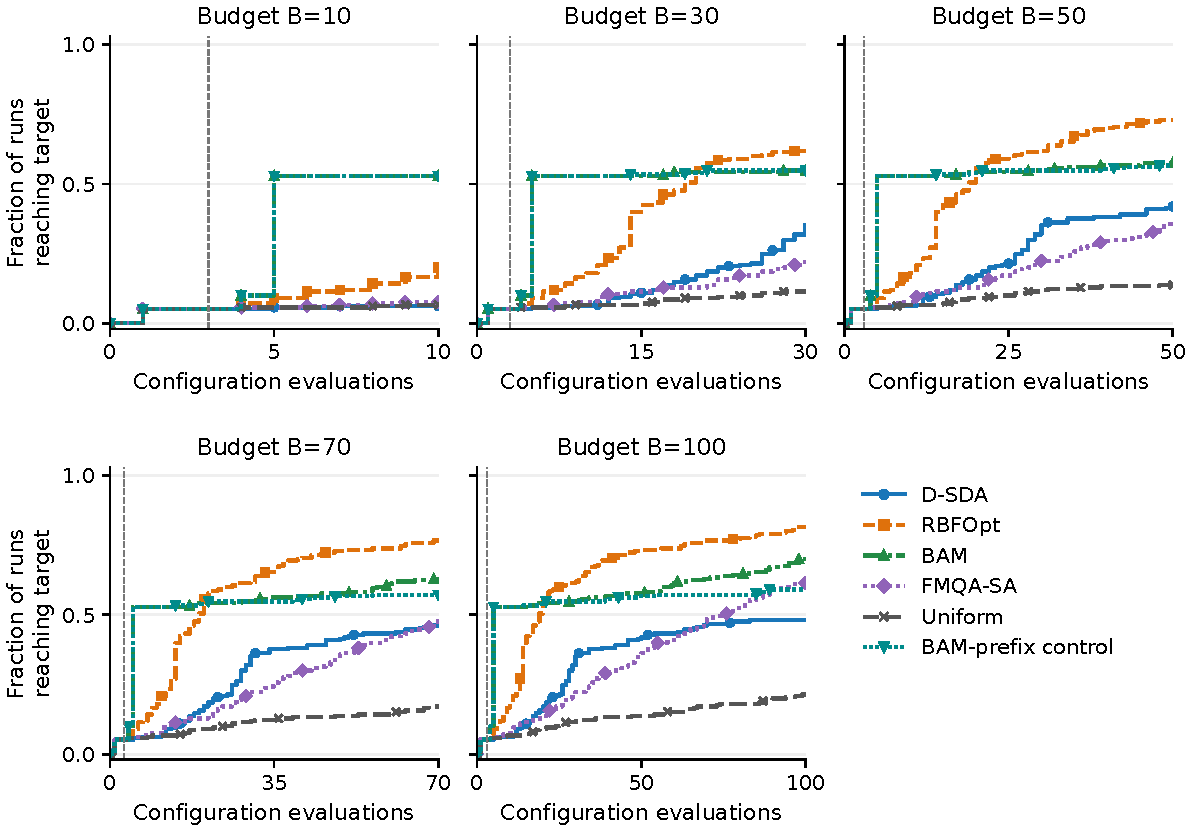
\includegraphics[width=\linewidth]{figures/figure_B_grid_evaluation_profiles.pdf}
\caption{Cumulative success profiles for 21 Grid-GDP functions and ten seeds per function at \(B=100\), following Equation~\eqref{eqn:absolute-evaluations}.
The target is the normalized reference value zero within \(10^{-5}\), as defined by Equation~\eqref{eqn:target}.
Each curve includes all 210 runs; initial and repeated evaluations count, and target misses remain in the denominator.
The dashed line marks the three shared initial evaluations.
Uniform sampling and the \texttt{BAM}-prefix control are defined in Section~\ref{sec:sampling-controls}.
\texttt{BAM} rises early, while \texttt{RBFOpt} reaches the largest final fraction at 100 evaluations.
\david{You cannot differetiate BAM and BAM prefix. I believe this color scheme is not colorblind friendly}
\albert{Distinguished BAM and its prefix control by solid versus dash-dot lines, filled versus open markers, and green versus black; curve values are unchanged.}
}
\label{fig:grid-profiles}
\end{figure}

\FloatBarrier

\subsection{Computational Comparison on Grid-GDP Problems}
\label{sec:grid-gdp-results}
Higher target-reaching rates do not necessarily correspond to shorter full-run completion times (Table~\ref{tab:grid-cost}).
At \(B=100\), \texttt{RBFOpt} has a median estimated full-run completion time of 70.81~s, compared with 24.08~s for \texttt{D-SDA} and 64.42~s for \texttt{BAM}.
\texttt{D-SDA} has negligible search overhead and can stop before exhausting the budget, while \texttt{RBFOpt} spends a median of 7.58~s on search.
For \texttt{FMQA-SA}, the median search component is 62.04~s, and the median completion estimate is 124.13~s.
Because Grid configurations fix both original coordinates, their measured evaluation costs primarily reflect model preparation, solver invocation, and verification.
\begin{table}[htbp]
\centering
\caption{Grid-GDP results at \(B=100\), with 210 runs per method (21 functions and ten seeds).
Target hits reach the normalized reference zero within \(10^{-5}\) (Equation~\eqref{eqn:target}).
Times are Q50 (median) [Q25, Q75] in seconds across all runs, including target misses, using linearly interpolated quartiles.
Summed configuration-evaluation cost includes the separately measured cost of every evaluation in the full run, including repeated configurations.
Search time excludes lookup processing; adding it to the summed configuration-evaluation cost gives estimated full-run completion time (Equation~\eqref{eqn:reconstructed-cost}).
Component quartiles need not sum to completion quartiles.
}
\label{tab:grid-cost}
\small
\begin{tabular}{lrrrr}\toprule
Method & Target hits & \shortstack{Full-run\\completion (s)} & \shortstack{Summed configuration-\\evaluation cost (s)} & \shortstack{Search\\time (s)}\\\midrule
\texttt{D-SDA} & 101/210 & \shortstack{24.08\\{[15.58, 49.49]}} & \shortstack{24.08\\{[15.58, 49.48]}} & \shortstack{0.0039\\{[0.0037, 0.0043]}} \\
\texttt{RBFOpt} & 171/210 & \shortstack{70.81\\{[54.83, 93.09]}} & \shortstack{60.84\\{[44.31, 82.15]}} & \shortstack{7.58\\{[4.12, 14.82]}} \\
\texttt{BAM} & 147/210 & \shortstack{64.42\\{[48.74, 81.67]}} & \shortstack{63.97\\{[48.34, 81.22]}} & \shortstack{0.43\\{[0.37, 0.51]}} \\
\texttt{FMQA-SA} & 129/210 & \shortstack{124.13\\{[105.57, 139.26]}} & \shortstack{62.34\\{[43.98, 77.52]}} & \shortstack{62.04\\{[61.58, 62.53]}} \\
Uniform & 45/210 & \shortstack{60.51\\{[43.33, 78.60]}} & \shortstack{60.51\\{[43.33, 78.59]}} & \shortstack{0.0026\\{[0.0026, 0.0027]}} \\
\texttt{BAM}-prefix control & 124/210 & \shortstack{61.81\\{[40.96, 78.33]}} & \shortstack{61.80\\{[40.95, 78.33]}} & \shortstack{0.0026\\{[0.0026, 0.0027]}} \\
\bottomrule
\end{tabular}
\end{table}

\texttt{D-SDA} and \texttt{BAM} nevertheless have zero observed hits on four and two functions, respectively; \texttt{RBFOpt} and \texttt{FMQA-SA} have at least one hit on every function at that evaluation budget.
Uniform has seven zero-hit functions, and the prefix control has two.

The conventional GDP comparisons report one selected result per problem and method; their iterations and subsolver calls are not equivalent to DFO callbacks.
The conventional GDP methods and their configurations are described in Section~\ref{sec:protocol}.
The direct Big-\(M\) and Hull reformulations solved with \texttt{SCIP} reach all 21 reference targets.
RIC and GLOA each reach 15 of the 21 Grid targets, while LOA reaches 14.
Numerically feasible solutions were saved for all 63 \texttt{GDPOpt} runs, with no execution errors reported (Supplementary Section~\ref{sec:supp-data}).
All three miss H\"older table, Michalewicz, and Shubert (historical variant).
Earlier diagnostic runs identified \texttt{GDPOpt} preprocessing rejections of independently feasible reference configurations; the same three problems miss their targets in the current runs.
Ten \texttt{GDPOpt} runs reach the target before terminating at the time limit.
Consequently, the measured completion time of a target-attaining run must be distinguished from a completed global-optimality certification.

\subsection{Process GDP Case Studies}
\label{sec:process-results}

\subsubsection{Target attainment}
Across the six \texttt{CSTR} sizes, \texttt{RBFOpt} reaches 45 of 60 targets, compared with 14 for \texttt{D-SDA} (Table~\ref{tab:process-targets}).
It has more target hits at every tested size under the stated size-dependent budgets.
For \texttt{Dynamic}, \texttt{RBFOpt} reaches all ten targets at every tested budget, starting at \(B=12\), where \texttt{D-SDA} reaches four.
\texttt{D-SDA} reaches all ten from \(B=30\) onward.

The method with the most target hits differs across process problems.
\texttt{BAM} reaches all ten targets on \texttt{CSTR5} at \(B=8\), compared with eight for \texttt{RBFOpt}.
On \texttt{Column} at \(B=13\), \texttt{D-SDA} reaches five of ten targets and \texttt{RBFOpt} four within the 64-configuration logical domain.
Across the ten seeds, final objectives range from 19346.1 to 19565.9 for \texttt{D-SDA} and from 19346.1 to 20491.9 for \texttt{RBFOpt}.
The only \texttt{Column} hits for \texttt{BAM} and uniform sampling occur at the shared initial target in seed 6.
On \texttt{Small Batch} at \(B=10\), \texttt{D-SDA} reaches eight targets, compared with five for \texttt{RBFOpt}.

\texttt{FMQA-SA} reaches 42 of 140 process targets, compared with 37 for uniform sampling.
Its aggregate gain over uniform is smaller here than on Grid.
Supplementary Section~\ref{sec:supp-proposals} reports fallback counts.
\begin{table}[htbp]
\centering
\caption{Reference-target attainment in the \texttt{IPOPT}-table process experiments.
Each cell lists target hits out of ten paired seeds, median search time, and [Q25, Q75] search time in seconds, from top to bottom.
Search times exclude configuration-evaluation costs and summarize all ten seeds.
The quartile ranges describe seed variability, not confidence intervals.
Bold counts mark the largest number of target hits in each row, including ties.
\david{include median and interval search times (not accounting for NLP solutions) for each method}
\albert{Added median and [Q25, Q75] search times from the completed 700-run comparison, excluding NLP evaluation costs and retaining all ten seeds per condition.}
}
\label{tab:process-targets}
\small
\begin{tabular}{@{}lrccccc@{}}\toprule
Case & Budget \(B\) & \texttt{D-SDA} & \texttt{RBFOpt} & \texttt{BAM} & \texttt{FMQA-SA} & Uniform \\
\midrule
\texttt{Column} & 13 & \makecell{\textbf{5}\\0.0153\\{[0.015, 0.0158]}} & \makecell{4\\0.226\\{[0.205, 0.239]}} & \makecell{1\\0.0177\\{[0.0168, 0.155]}} & \makecell{4\\6.85\\{[6.81, 6.89]}} & \makecell{1\\0.00716\\{[0.00711, 0.00748]}} \\
\texttt{CSTR5} & 8 & \makecell{2\\0.0136\\{[0.0135, 0.014]}} & \makecell{8\\0.0596\\{[0.059, 0.0597]}} & \makecell{\textbf{10}\\0.036\\{[0.0151, 0.0816]}} & \makecell{3\\3.66\\{[3.64, 3.67]}} & \makecell{4\\0.0046\\{[0.00387, 0.00478]}} \\
\texttt{CSTR10} & 15 & \makecell{2\\0.0179\\{[0.016, 0.0193]}} & \makecell{\textbf{6}\\0.302\\{[0.288, 0.315]}} & \makecell{1\\0.137\\{[0.126, 0.158]}} & \makecell{2\\8\\{[7.98, 8.08]}} & \makecell{1\\0.00807\\{[0.00772, 0.00812]}} \\
\texttt{CSTR15} & 22 & \makecell{2\\0.0216\\{[0.0201, 0.0228]}} & \makecell{\textbf{7}\\1\\{[0.492, 3.26]}} & \makecell{1\\0.15\\{[0.14, 0.162]}} & \makecell{1\\12.4\\{[12.3, 12.4]}} & \makecell{2\\0.0113\\{[0.0108, 0.0116]}} \\
\texttt{CSTR20} & 29 & \makecell{3\\0.026\\{[0.022, 0.0292]}} & \makecell{\textbf{7}\\2.82\\{[0.632, 4.01]}} & \makecell{2\\0.167\\{[0.165, 0.313]}} & \makecell{1\\16.9\\{[16.8, 16.9]}} & \makecell{2\\0.0139\\{[0.0121, 0.0148]}} \\
\texttt{CSTR25} & 36 & \makecell{3\\0.0334\\{[0.0288, 0.0361]}} & \makecell{\textbf{8}\\2.47\\{[1.86, 4.43]}} & \makecell{2\\0.401\\{[0.392, 0.449]}} & \makecell{1\\21.3\\{[21.3, 21.4]}} & \makecell{1\\0.0161\\{[0.0147, 0.0186]}} \\
\texttt{CSTR30} & 43 & \makecell{2\\0.0586\\{[0.0572, 0.0645]}} & \makecell{\textbf{9}\\4.99\\{[2.95, 10.3]}} & \makecell{2\\0.425\\{[0.404, 0.451]}} & \makecell{1\\25.8\\{[25.7, 26]}} & \makecell{1\\0.0241\\{[0.0224, 0.0257]}} \\
\texttt{Small Batch} & 10 & \makecell{\textbf{8}\\0.0136\\{[0.0131, 0.0139]}} & \makecell{5\\0.17\\{[0.159, 0.18]}} & \makecell{2\\0.0169\\{[0.0161, 0.0191]}} & \makecell{6\\4.87\\{[4.86, 4.89]}} & \makecell{4\\0.00536\\{[0.00506, 0.00545]}} \\
\texttt{Dynamic} & 12 & \makecell{4\\0.0152\\{[0.0149, 0.0153]}} & \makecell{\textbf{10}\\0.186\\{[0.182, 0.189]}} & \makecell{0\\0.0173\\{[0.0172, 0.0174]}} & \makecell{2\\6.16\\{[6.14, 6.2]}} & \makecell{0\\0.00589\\{[0.0054, 0.00658]}} \\
\texttt{Dynamic} & 15 & \makecell{5\\0.0172\\{[0.0162, 0.0173]}} & \makecell{\textbf{10}\\0.296\\{[0.291, 0.321]}} & \makecell{3\\0.139\\{[0.128, 0.156]}} & \makecell{3\\8.04\\{[8.01, 8.09]}} & \makecell{3\\0.0074\\{[0.00622, 0.0076]}} \\
\texttt{Dynamic} & 20 & \makecell{8\\0.0184\\{[0.0178, 0.0202]}} & \makecell{\textbf{10}\\0.367\\{[0.355, 0.381]}} & \makecell{3\\0.143\\{[0.13, 0.156]}} & \makecell{3\\11.2\\{[11.1, 11.2]}} & \makecell{3\\0.00987\\{[0.00927, 0.00991]}} \\
\texttt{Dynamic} & 30 & \makecell{\textbf{10}\\0.0219\\{[0.018, 0.0233]}} & \makecell{\textbf{10}\\7.61\\{[4.88, 13.7]}} & \makecell{4\\0.355\\{[0.204, 0.364]}} & \makecell{4\\17.4\\{[17.2, 17.5]}} & \makecell{4\\0.0141\\{[0.0135, 0.0145]}} \\
\texttt{Dynamic} & 37 & \makecell{\textbf{10}\\0.023\\{[0.0176, 0.0243]}} & \makecell{\textbf{10}\\10.1\\{[5.25, 14.2]}} & \makecell{7\\0.376\\{[0.364, 0.383]}} & \makecell{5\\21.7\\{[21.6, 21.8]}} & \makecell{5\\0.0173\\{[0.0171, 0.0174]}} \\
\texttt{Dynamic} & 50 & \makecell{\textbf{10}\\0.0223\\{[0.0176, 0.0238]}} & \makecell{\textbf{10}\\26.3\\{[17, 37.2]}} & \makecell{\textbf{10}\\0.732\\{[0.685, 0.751]}} & \makecell{6\\29.8\\{[29.7, 30.1]}} & \makecell{6\\0.0233\\{[0.0229, 0.0235]}} \\
\bottomrule
\end{tabular}
\par\vspace{3pt}
\end{table}

Figure~\ref{fig:process-evaluations} shows the first target-attaining evaluation on successful recorded runs, with misses and execution failures retained in the denominator.
\begin{figure}[htbp]
\centering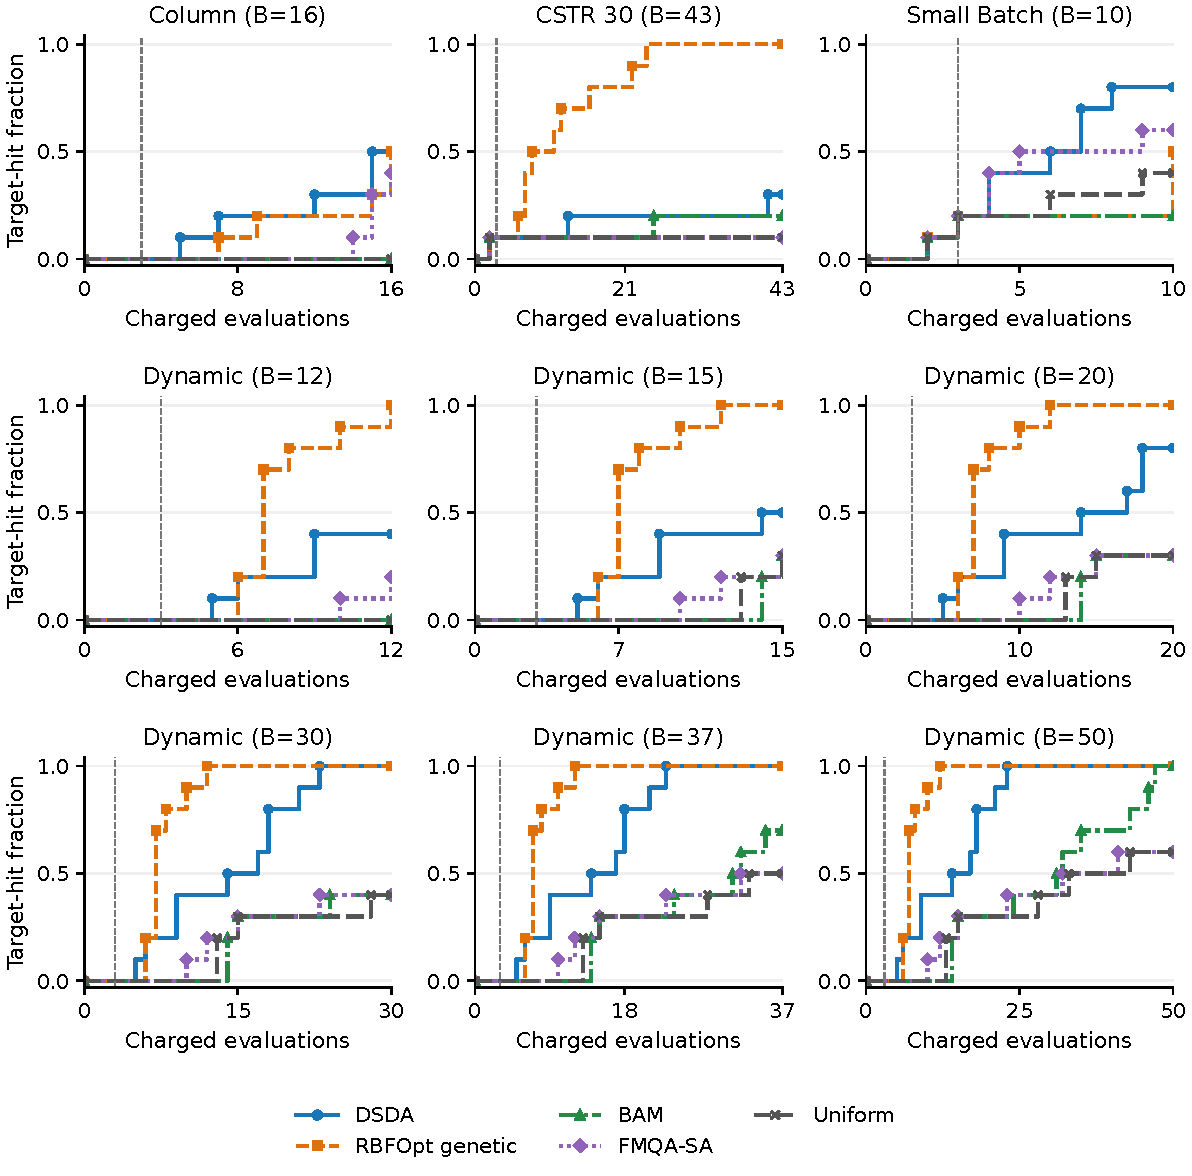
\includegraphics[width=\linewidth]{figures/process_evaluation_profiles.pdf}
\caption{Cumulative target attainment versus charged evaluations for nine illustrative process conditions, using the wrapper-reported success definition in Section~\ref{sec:metrics}.
Every method-condition group retains all ten seeds, including target misses.
Initialization, unsuccessful evaluations, and repeated callbacks consume the budget.
Steps mark the first accepted target observation on successful runs.
The gray vertical line at three evaluations marks the end of the shared initialization.
Line styles and markers distinguish methods.
All 14 conditions appear in Table~\ref{tab:process-targets}.}
\label{fig:process-evaluations}
\end{figure}

\subsubsection{Computational cost}

For \texttt{Dynamic} at \(B=50\), search overhead contributes 42.7\% of the mean estimated completion time for \texttt{RBFOpt}, compared with less than 0.2\% for \texttt{D-SDA}.
\texttt{Dynamic} \texttt{D-SDA} executes 221 callbacks across ten \(B=50\) runs, compared with 500 for each of \texttt{RBFOpt}, \texttt{BAM}, and \texttt{FMQA-SA}.
Its lower cost reflects shorter paths as well as low search overhead; unsuccessful candidates are evaluated and charged within the common box.

On \texttt{Column}, median completion estimates are 35.44~s for \texttt{D-SDA} and 54.60~s for \texttt{RBFOpt} (Figure~\ref{fig:process-completion}).
For \texttt{Dynamic} at \(B=30\), \texttt{RBFOpt} reaches all ten targets in fewer evaluations than \texttt{D-SDA} (Figure~\ref{fig:process-evaluations}).
Its median estimated full-run completion time is nevertheless higher: 34.19~s versus 26.62~s (Figure~\ref{fig:process-completion}).
Earlier target discovery therefore need not reduce full-run cost, which includes subsequent evaluations and search overhead.
At the smaller budget \(B=12\), \texttt{RBFOpt} reaches all ten targets with a median completion estimate of 12.29~s.

\begin{figure}[htbp]
\centering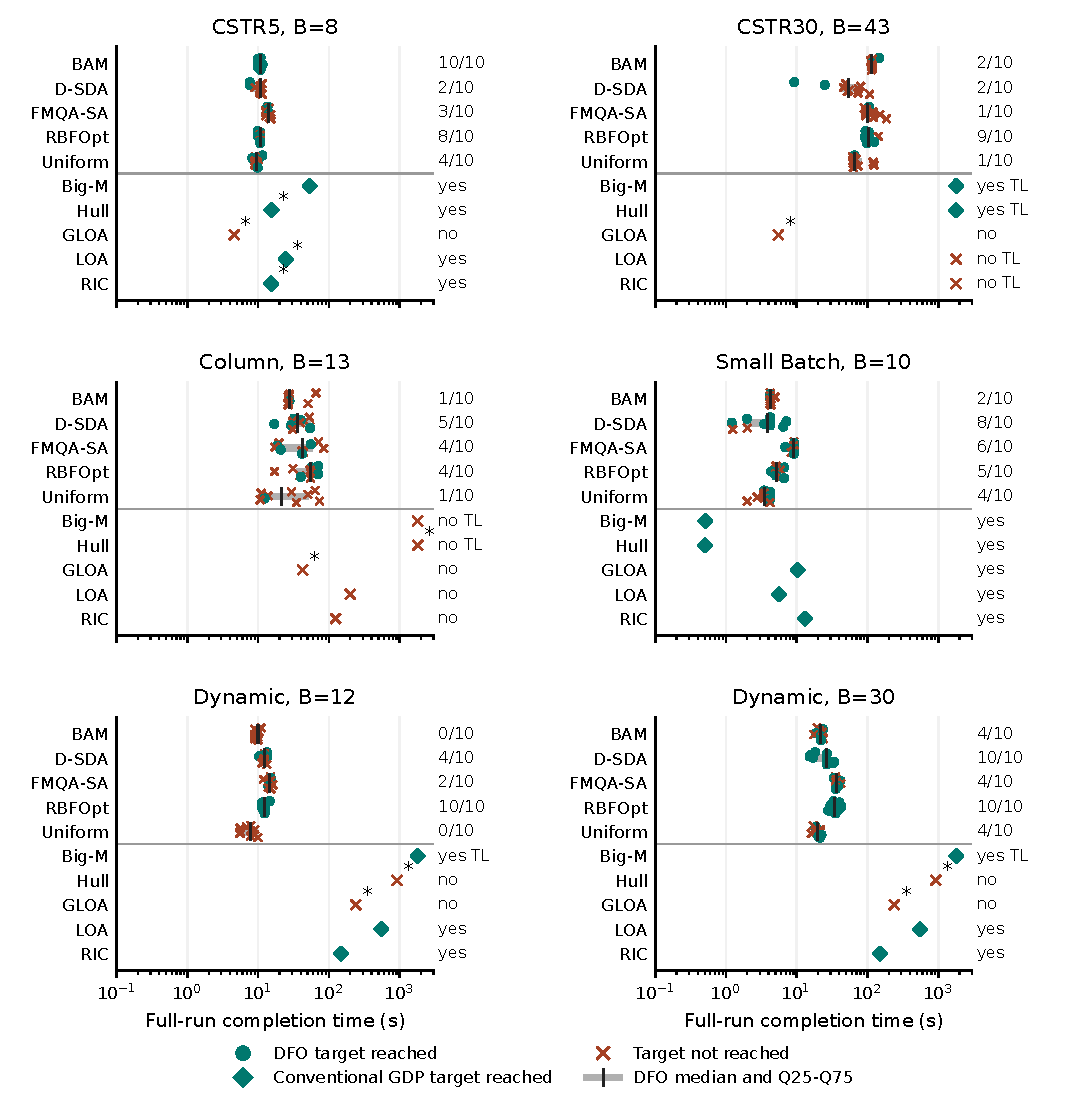
\includegraphics[width=\linewidth]{figures/process_joint_completion.pdf}
\caption{Joint full-run completion-time comparison for six process conditions.
DFO times are reconstructed using Equation~\eqref{eqn:reconstructed-cost}; conventional GDP times are measured and include model preparation.
Dots show individual successful DFO runs, diamonds successful single conventional runs, and crosses target misses under the rules in Section~\ref{sec:metrics}.
Gray segments and ticks show Q25--Q75 and medians across all ten DFO seeds; right-hand labels give hits out of ten or the single-run outcome.
TL denotes reported time-limit termination; asterisks mark the bound inconsistencies discussed in Section~\ref{sec:bound-audit} of the supplement.
The logarithmic axis retains recorded completion times, not first-target times.
The two Dynamic panels reuse the same conventional observations.
}
\label{fig:process-completion}
\end{figure}

\david{If the NLPs or times are comparable to the times in Figures 2 and 3, include them as a vertical bar to contextualize the result (vertical bar is equivalent to them having solved the problem). Units for time (s) are missing. Highlight the best result per row in bold. If the time limit is reached, then put the time as 1800+ (in some cases it is 1791 $\le$ 1800)}
\albert{Added the joint completion-time comparison to Figure 3 and moved the detailed table to the supplement, retaining all DFO seeds and single conventional observations.
Time units and bold row minima are shown; TL identifies limit terminations while preserving measured times rather than replacing them with 1800.
Removed duplicate supplementary panels and the unused cumulative time-profile definition.}

Supplementary Table~\ref{tab:process-tts99} reports median estimated full-run completion times for all 14 conditions; Supplementary Figure~\ref{fig:joint-remaining-completion} shows the eight conditions not included in Figure~\ref{fig:process-completion}.
For \texttt{CSTR30}, \texttt{RBFOpt} reaches nine targets with a median completion estimate of 101.96~s.
\texttt{D-SDA} reaches two targets at 53.12~s, and \texttt{BAM} reaches two at 115.41~s.
The single Big-\(M\) and Hull runs reach the \texttt{CSTR30} target at completion times of 1,791.82 and 1,792.56~s, while the three GDPopt runs miss it (Figure~\ref{fig:process-completion}).

\FloatBarrier

Supplementary Table~\ref{tab:full-gdp} reports the detailed results of five conventional GDP methods on nine process models.
Of the 45 runs, 43 return solutions that pass the original-GDP residual test at \(10^{-5}\).
Big-\(M\) returns no accepted feasible solution for \texttt{CSTR15} or \texttt{Column} within the time limit.
Hull reaches the most reference targets, succeeding on seven of the nine models.
RIC, LOA, and Big-\(M\) each reach five targets, while GLOA reaches only the \texttt{Small Batch} target.
RIC and LOA reach the \texttt{Dynamic} target but miss those for \texttt{CSTR10} and \texttt{CSTR25}.
\david{you usually do not use fractions in a sentence, and the sentence just reads like a laundry list. Have more prose}
\albert{Replaced the fraction list with a prose summary of the updated results.}
These single-run results do not establish success probabilities or global optimality.

All five methods attain the \texttt{Small Batch} reference.
Big-\(M\) and Hull complete in 0.51 and 0.50~s, respectively, compared with median DFO completion estimates ranging from 3.49 to 9.09~s.
Direct reformulation is faster on this benchmark and reaches the target in both runs (Figure~\ref{fig:process-completion}).

All six \texttt{CSTR} GLOA runs report \texttt{optimal}, but their objective differences from the reference exceed \(10^{-5}\max\{1,|f_{\mathrm{ref}}|\}\).
\david{help the reader, remind them what this means and the epsilon it represents}
\albert{Stated the reference-target tolerance explicitly.}
Their reported lower bounds exceed independently checked feasible objectives.
The \texttt{Dynamic} Hull run has the same inconsistency: its lower bound is \(-196.931\), while the saved Big-\(M\) point has objective \(-212.009\).
That point also passes a check against the reconstructed Hull formulation (Supplementary Section~\ref{sec:bound-audit}).
The uniform bound check flags 21 results, including eight smaller exceedances of 1.09-3.54 times the comparison tolerance.
The flags distinguish numerical consistency from target attainment and reported termination; they do not establish exact feasibility or a solver defect.

A separate \texttt{CSTR15} check using \texttt{IPOPT} 3.14.19 retained the archived LOA witness W03's discrete configuration and starting values (Supplementary Section~\ref{sec:bound-audit})~\citep{rbfoptTestArchive}.
\david{Why would a reader know that Dantzig is a computer? SInce we refer to all computational results from that computer, you can just avoid mentioning its name}
\albert{Removed the machine name.}
The returned objective was \(2.82939\), with the maximum unscaled original-GDP violation \(1.11\times10^{-16}\), passing a residual target \(10^{-8}\).
The new GLOA lower bound exceeds this previously validated objective by \(0.732565\), approximately \(2.59\times10^4\) times the audit tolerance.
The discrepancy therefore persists against the tighter feasibility check, although its cause remains unresolved.

\FloatBarrier

\subsection{Discussion}
\label{sec:cross-benchmark}
On the tested GDP external integer domains, alternative black-box methods improved target-reaching rates over budget-limited \texttt{D-SDA} in some cases.
The gains depend on the search method, problem, and budget.

On the grid instances, \texttt{BAM} leads with ten evaluations, while \texttt{RBFOpt} leads at the tested budgets of thirty evaluations or more.
\texttt{BAM}'s early hits come from initial sampling, while its later search adds hits beyond the prefix control.
For nine Grid functions, the domain center satisfies the target criterion and is visited by \texttt{BAM} at its fifth evaluation.
On the process cases, \texttt{RBFOpt} improves on \texttt{D-SDA} for \texttt{CSTR} and low-budget \texttt{Dynamic}, while \texttt{D-SDA} leads on \texttt{Column} and \texttt{Small Batch}.
For \texttt{CSTR30}, the target lies at the upper corner of the domain, while seven of the ten \texttt{D-SDA} runs stop elsewhere with no improving neighbor.
In \texttt{Column}, four of the five successful \texttt{D-SDA} runs reach the target in one or two improving moves, and the fifth starts at the target.
\texttt{FMQA-SA} also improves over uniform sampling at larger Grid budgets, with smaller aggregate gains in the process comparisons.
\david{Provide more details here: why do some instances benefit some solvers? What's the hidden structure?}
\albert{Added evidence from the saved records on Grid target locations, CSTR30 local stopping, and Column improvement paths.}

Increasing the evaluation budget does not improve target-reaching rates equally across methods.
On \texttt{Dynamic}, \texttt{RBFOpt} reaches the target in all ten runs at \(B=12\), but its median estimated completion time increases from 12.29~s at \(B=12\) to 65.14~s at \(B=50\).
For \texttt{D-SDA}, the number of successful runs increases from four at \(B=12\) to ten at \(B=30\), with little further change in completion cost at larger budgets.
Increasing the budget from \(B=30\) to \(B=50\) improves the target counts for \texttt{BAM} from four to ten and for \texttt{FMQA-SA} from four to six, at higher estimated completion costs.
\david{This is to be expected; by preprocessing, you do not solve problems. But mention which solvers stall and which keep growing with more iterations; also mention if there is a tradeoff search time and solution quality.}
\albert{Added the Dynamic budget comparison showing where target-reaching rates improve or plateau and how completion costs change.}

The comparison with conventional GDP methods also depends on the problem.
On \texttt{Small Batch}, direct Big-\(M\) and Hull reach the target in 0.51 and 0.50~s, respectively, compared with median estimated DFO completion times ranging from 3.49 to 9.09~s.
On \texttt{CSTR30}, \texttt{RBFOpt} reaches the target in nine of ten runs with a median estimated completion time of 101.96~s, while the single Big-\(M\) and Hull runs reach it with completion times of approximately 1,792~s.
These results show a benefit of configuration search on \texttt{CSTR30}, while direct reformulation is more effective on \texttt{Small Batch}.
\david{This is the usual AI warning about scalability; rather, say which cases benefited from the conventional GDP solution models than the integration with DFOs, and in the conclusion you mention this as recommendations for future instances}
\albert{Replaced the generic scalability warning with the Small Batch and CSTR30 comparisons and added their implications to the conclusions.}

\section{Conclusions}
This study compared black-box methods for GDP configuration search using an existing external integer representation.
Alternatives to budget-limited \texttt{D-SDA} improved target-reaching rates in some cases, with benefits depending on the problem and evaluation budget.
On \texttt{Dynamic}, \texttt{RBFOpt} returned the same target value in all ten runs at every tested budget.
On \texttt{Column}, \texttt{D-SDA} reached the target more often and returned final objective values within a narrower range than \texttt{RBFOpt} across the ten seeds.
Higher target-reaching rates did not consistently correspond to shorter estimated full-run completion times, so method selection should consider both measures.
\david{Sure, this is obvious; any deeper insights? How about the fact that they are stochastic? That you would get different solutions when running them separately; were they spread out?}
\albert{Added the contrasting seed-level results for Dynamic and Column to describe consistency in target discovery and variation in final solution quality.}

Direct reformulation was faster on \texttt{Small Batch}, while \texttt{RBFOpt} reached the \texttt{CSTR30} target in nine of ten runs at lower estimated completion costs than the successful direct reformulations.
These results support considering DFO configuration search when good feasible solutions are needed and solving the full algebraic model is costly.
The approach could also be useful when configuration evaluations come from simulations and explicit subproblem equations are unavailable.
\david{how is this a conclusion? What did you learn from all these experiments?}
\albert{Revised the paragraph to explain what the Small Batch and CSTR30 comparisons teach us and identify simulation-based subproblems as a future application.}

\section{Acknowledgement}
The authors acknowledge and express sincere gratitude to the Davidson School of Chemical Engineering at Purdue University for providing a supportive research environment and funding.

\section*{Data and code availability}
The code and data are available in the \href{https://github.com/SECQUOIA/Black-Box-for-GDP/tree/49d4bcbeb10fe49b74fe2333d27829046e93bf03}{Black-Box-for-GDP repository}~\citep{rbfoptTestArchive}.
Supplementary Section~\ref{sec:supp-data} identifies the archived inputs, including the CSTR updates, Column logical-domain runs, and conventional GDP comparisons.

\section*{Declaration of generative AI and AI-assisted technologies in the manuscript preparation process}
The authors used ChatGPT and Codex (OpenAI), including the GPT-6 Astra model, to assist with drafting, organizing, and revising the manuscript and developing analysis and plotting code.
\david{which models?}
\albert{Specified GPT-6 Astra and described AI-assisted code development and verification in the Methods.}
The resulting text and code were checked and revised by the authors, who remain responsible for the article's content.

\bibliographystyle{elsarticle-harv}
\bibliography{reference}
% Include the existing supplementary source in this review PDF.
\def\manuscriptwithsupplement{1}
\ifdefined\manuscriptwithsupplement
\clearpage
\begingroup
\normalsize
\setcounter{section}{0}
\setcounter{table}{0}
\setcounter{figure}{0}
\setcounter{equation}{0}
\renewcommand{\thesection}{S\arabic{section}}
\renewcommand{\thetable}{S\arabic{table}}
\renewcommand{\thefigure}{S\arabic{figure}}
\renewcommand{\theequation}{S\arabic{equation}}
\renewcommand{\theHsection}{supp.\arabic{section}}
\renewcommand{\theHtable}{supp.\arabic{table}}
\renewcommand{\theHfigure}{supp.\arabic{figure}}
\renewcommand{\theHequation}{supp.\arabic{equation}}
\setlength{\emergencystretch}{2em}
\clubpenalty=10000
\widowpenalty=10000
\begin{center}
{\LARGE Supplementary Material:\\Benchmark Definitions, Execution Protocol, and Uncertainty\par}
\end{center}
\else
\documentclass{article}
\usepackage[T1]{fontenc}
\usepackage[utf8]{inputenc}
\usepackage[letterpaper,margin=1in]{geometry}
\usepackage{amsmath,amssymb,booktabs,placeins,xurl}
\usepackage{longtable,pdflscape,graphicx}
\renewcommand{\thefigure}{S\arabic{figure}}
\usepackage[authoryear,round,sort]{natbib}
\usepackage[hidelinks]{hyperref}
\renewcommand{\thetable}{S\arabic{table}}
\renewcommand{\theequation}{S\arabic{equation}}
\renewcommand{\thesection}{S\arabic{section}}
\setlength{\emergencystretch}{2em}
\clubpenalty=10000
\widowpenalty=10000
\title{Supplementary Material:\\Benchmark Definitions, Execution Protocol, and Uncertainty}
\author{}
\date{}
\setlength{\emergencystretch}{2em}
\begin{document}
\maketitle
\vspace{-2em}
\fi
The Grid-GDP functions are adapted from the Quantum Hamiltonian Descent collection; each instance is defined by its implemented expression and domain rather than its conventional name~\citep{qhdBenchmarks,rbfoptTestArchive}.

\section{Coordinate domains and normalization}\label{sec:supp-domains}
The coordinate mapping and objective normalization follow Section~\ifdefined\manuscriptwithsupplement\ref{sec:grid-gdp-formulation}\else3.1\fi{} of the main paper.
Both coordinate endpoints are included, and \(L\) and \(U\) are the minimum and maximum over the 961 lattice points.
All trigonometric arguments are in radians.
Full-precision normalization constants and target coordinates are archived in \nolinkurl{grid_inventory.json} (Section~\ref{sec:supp-data}).

\begin{table}[htbp]
\centering\small
\caption{Grid-GDP benchmark domains and target-set sizes.
Each problem uses a \(31\times31\) lattice with 961 configurations and 62 Boolean indicators.
\(n_{\rm target}\) counts lattice points with normalized objective \(F\leq10^{-5}\).}
\label{tab:grid-domains}
\begin{tabular}{llll}\toprule
Function & \(x\) domain & \(y\) domain & \(n_{\rm target}\)\\\midrule
Ackley & \([-5,5]\) & \([-5,5]\) & 1\\
Alpine 1 & \([0,10]\) & \([0,10]\) & 1\\
Alpine 2 & \([0,1000]\) & \([0,1000]\) & 1\\
Bohachevsky 2 & \([-100,100]\) & \([-100,100]\) & 1\\
Three-hump camel & \([-5,5]\) & \([-5,5]\) & 1\\
Csendes (squared variant) & \([-1,1]\) & \([-1,1]\) & 36\\
Deflected corrugated spring & \([0,10]\) & \([0,10]\) & 1\\
Drop-Wave & \([-5.12,5.12]\) & \([-5.12,5.12]\) & 1\\
Easom & \([-10,10]\) & \([-10,10]\) & 1\\
Griewank & \([-600,600]\) & \([-600,600]\) & 1\\
H\"older table & \([-10,10]\) & \([-10,10]\) & 4\\
Hosaki & \([0,5]\) & \([0,6]\) & 1\\
L\'evy & \([-10,10]\) & \([-10,10]\) & 2\\
L\'evy 13 & \([-10,10]\) & \([-10,10]\) & 4\\
Michalewicz & \([0,\pi]\) & \([0,\pi]\) & 1\\
Rastrigin & \([-5.12,5.12]\) & \([-5.12,5.12]\) & 1\\
Rosenbrock & \([-2,2]\) & \([-1,3]\) & 2\\
Shubert (historical variant) & \([0,10]\) & \([0,10]\) & 1\\
Styblinski--Tang & \([-5,5]\) & \([-5,5]\) & 1\\
Sum of squares & \([-10,10]\) & \([-10,10]\) & 1\\
Xin-She Yang 3 (historical variant) & \([-20,20]\) & \([-20,20]\) & 870\\\bottomrule
\end{tabular}
\end{table}

\FloatBarrier % \clearpage
\section{Grid-GDP objective functions}\label{sec:supp-objectives}
The implemented functions below use the domains in Table~\ref{tab:grid-domains}~\citep{rbfoptTestArchive}.

\subsection*{1. Ackley}
\begin{equation}\label{eq:supp-ackley}
\begin{aligned}
f(x,y)={}&-20\exp\!\left(-0.2\sqrt{\frac{x^2+y^2}{2}}\right)\\
&-\exp\!\left(\frac{\cos(2\pi x)+\cos(2\pi y)}{2}\right)+20+e.
\end{aligned}
\end{equation}

\subsection*{2. Alpine 1}
\begin{equation}\label{eq:supp-alpine1}
f(x,y)=|x\sin x+0.1x|+|y\sin y+0.1y|.
\end{equation}

\subsection*{3. Alpine 2}
\begin{equation}\label{eq:supp-alpine2}
f(x,y)=-\sqrt{xy}\,\sin x\sin y.
\end{equation}

\subsection*{4. Bohachevsky 2}
\begin{equation}\label{eq:supp-bohachevsky2}
f(x,y)=x^2+2y^2-0.3\cos(3\pi x)\cos(4\pi y)+0.3.
\end{equation}

\subsection*{5. Three-hump camel}
\begin{equation}\label{eq:supp-camel3}
f(x,y)=2x^2-1.05x^4+\frac{x^6}{6}+xy+y^2.
\end{equation}

\subsection*{6. Csendes (squared variant)}
\begin{equation}\label{eq:supp-csendes}
f(x,y)=c(x)+c(y),\qquad
c(t)=\begin{cases}
t^6\bigl[2+\sin(1/t)\bigr]^2,&t\ne0,\\
0,&t=0.
\end{cases}
\end{equation}
The GDP uses branch-fixed auxiliaries \(r_t=1/t\) for \(t\ne0\) and \(r_t=0\) otherwise, avoiding division by zero without an epsilon shift.

\subsection*{7. Deflected corrugated spring}
With \(r=\sqrt{(x-5)^2+(y-5)^2}\),
\begin{equation}\label{eq:supp-spring}
f(x,y)=0.1r^2-\cos(5r).
\end{equation}

\subsection*{8. Drop-Wave}
\begin{equation}\label{eq:supp-dropwave}
f(x,y)=-\frac{1+\cos\!\left(12\sqrt{x^2+y^2}\right)}{0.5(x^2+y^2)+2}.
\end{equation}

\subsection*{9. Easom}
\begin{equation}\label{eq:supp-easom}
f(x,y)=-\cos x\cos y\,\exp\!\left(-[(x-\pi)^2+(y-\pi)^2]\right).
\end{equation}

\subsection*{10. Griewank}
\begin{equation}\label{eq:supp-griewank}
f(x,y)=\frac{x^2+y^2}{4000}-\cos x\cos\!\left(\frac{y}{\sqrt{2}}\right)+1.
\end{equation}

\subsection*{11. H\"older table}
\begin{equation}\label{eq:supp-holder}
f(x,y)=-\left|\sin x\cos y\,
\exp\!\left(\left|1-\frac{\sqrt{x^2+y^2}}{\pi}\right|\right)\right|.
\end{equation}

\subsection*{12. Hosaki}
\begin{equation}\label{eq:supp-hosaki}
f(x,y)=\left(1-8x+7x^2-\frac{7}{3}x^3+\frac14x^4\right)y^2\exp(-y).
\end{equation}

\FloatBarrier % \clearpage
\subsection*{13. L\'evy}
Define \(w_x=1+(x-1)/4\) and \(w_y=1+(y-1)/4\).
Then
\begin{equation}\label{eq:supp-levy}
\begin{aligned}
f(x,y)={}&\sin^2(\pi w_x)\\
&+(w_x-1)^2\bigl[1+10\sin^2(\pi w_x+1)\bigr]\\
&+(w_y-1)^2\bigl[1+\sin^2(2\pi w_y)\bigr].
\end{aligned}
\end{equation}

\subsection*{14. L\'evy 13}
\begin{equation}\label{eq:supp-levy13}
\begin{aligned}
f(x,y)={}&\sin^2(3\pi x)+(x-1)^2\bigl[1+\sin^2(3\pi y)\bigr]\\
&+(y-1)^2\bigl[1+\sin^2(2\pi y)\bigr].
\end{aligned}
\end{equation}

\subsection*{15. Michalewicz}
\begin{equation}\label{eq:supp-michalewicz}
f(x,y)=-\sin x\,\sin^{20}\!\left(\frac{x^2}{\pi}\right)
-\sin y\,\sin^{20}\!\left(\frac{2y^2}{\pi}\right).
\end{equation}

\subsection*{16. Rastrigin}
\begin{equation}\label{eq:supp-rastrigin}
f(x,y)=x^2-10\cos(2\pi x)+y^2-10\cos(2\pi y)+20.
\end{equation}

\subsection*{17. Rosenbrock}
\begin{equation}\label{eq:supp-rosenbrock}
f(x,y)=(1-x)^2+100(y-x^2)^2.
\end{equation}

\subsection*{18. Shubert (historical variant)}
\begin{equation}\label{eq:supp-shubert}
\begin{aligned}
f(x,y)={}&\bigl[\cos(2x+1)+2\cos(3x+2)+3\cos(4x+3)\bigr]\\
&\times\bigl[\cos(2y+1)+\cos(y+2)\bigr].
\end{aligned}
\end{equation}

\FloatBarrier % \clearpage
\subsection*{19. Styblinski--Tang}
\begin{equation}\label{eq:supp-styblinski}
f(x,y)=\frac{1}{78}\,\frac12
\left(x^4-16x^2+5x+y^4-16y^2+5y\right).
\end{equation}

\subsection*{20. Sum of squares}
\begin{equation}\label{eq:supp-squares}
f(x,y)=x^2+2y^2.
\end{equation}

\subsection*{21. Xin-She Yang 3 (historical variant)}
\begin{equation}\label{eq:supp-xin}
f(x,y)=\exp\!\left(-\left[\left(\frac{x}{15}\right)^6+y^6\right]\right)
+2\exp\!\left(-(x^2+y^2)\right)\cos^2x\cos^2y.
\end{equation}

\FloatBarrier % \clearpage
\section{Executable protocol and implementation settings}\label{sec:supp-protocol}

Python and NumPy use the job seed, and \texttt{RBFOpt} also receives \nolinkurl{rand_seed}.
\texttt{BAM} exposes no separate native random-seed option: its process wrapper seeds Python/NumPy, while the Grid seed identifies the common initial design.
\texttt{FMQA-SA} uses three NumPy \nolinkurl{SeedSequence(seed)} streams for FM initialization, annealing, and uniform unseen-point fallback; each training or annealing invocation draws a seed from its stream.
\texttt{PyTorch} uses deterministic CPU operations and one thread.

Grid \texttt{D-SDA} enumerates \(L_\infty\) neighbors lexicographically from \((-1,0,1)\), excluding the zero direction and out-of-bounds points; ties select the first point.

The \texttt{RBFOpt} options are \nolinkurl{rbf=auto}, \nolinkurl{global_search_method=genetic}, \nolinkurl{do_init_strategy=False}, \nolinkurl{ga_base_population_size=400}, and \nolinkurl{ga_num_generations=20}.

\texttt{BAM} receives \nolinkurl{x0=None} and \nolinkurl{max_evals}=B-3; its local models use \texttt{ALAMO}/\texttt{BARON}, whose internal versions are not reported by the package.

The \texttt{FMQA-SA} time limit is checked between operations and through training/sampling callbacks.
Each FM uses identity activation, zero bias, and normal initial weights with mean zero and standard deviation \(0.01\).
Training uses Adam~\citep{kingma2015adam}, 1,000 full-batch epochs, mean squared error, and learning rate \(0.01\).
Coordinate \(\xi_j\) uses \(\lfloor\log_2 u_j\rfloor+1\) unsigned bits, where \(u_j>0\) is its upper bound; QUBO coefficients are divided by the largest absolute entry of the quadratic matrix.
D-Wave's \texttt{SimulatedAnnealingSampler} in \texttt{dwave-samplers} 1.6.0 uses 100 reads, 1,000 sweeps, and a geometric inverse-temperature schedule~\citep{dwaveSamplers}.
All process workers and the Grid \texttt{FMQA-SA} worker have a 2,100 s watchdog.
The Grid \texttt{RBFOpt}/\texttt{BAM} trace watchdogs are disabled (\nolinkurl{max_run_seconds=0}); archived Grid \texttt{D-SDA} uses budget, target, or local-search termination without an additional method-clock limit.

\subsection{Versions and independently timed process evaluations}\label{sec:supp-acceptance}
The recorded Python version is 3.11.16; other versions are given in the main paper\ifdefined\manuscriptwithsupplement\space(Section~\ref{sec:protocol})\fi.

The conventional GDP process models retain their archived initializations, including constructor defaults for \texttt{CSTR30}; the updated DFO evaluation table is identified separately in Section~\ref{sec:supp-data}.

The acceptance rule in \nolinkurl{gdp_models/evaluation.py} requires all of the following: a finite objective; termination in \{\texttt{optimal}, \texttt{locallyOptimal}, \texttt{globallyOptimal}\}; solver status other than \texttt{error} or \texttt{aborted}; interface status \texttt{SOLVESTAT}=1 and \texttt{MODELSTAT}\(\in\{1,2\}\); and a finite maximum primal violation no greater than \(10^{-5}\).
Time-limit, iteration-limit, evaluation-limit, and error outcomes are not accepted, even if a finite feasible candidate is available.

The primal check uses unscaled violations of original constraints and initialized-variable bounds, including constraint rows deactivated during preprocessing.
Nonfinite objectives, constraint bodies, or initialized-variable values preclude acceptance; unused uninitialized variables are skipped.
Preprocessing rejection or worker failure supplies no accepted objective.

The \texttt{CSTR} initializer \nolinkurl{cstr_box_ipopt.py:initialize_feasible} runs after preprocessing and checks the mass-balance/zero-recycle start at \(10^{-8}\) without changing constraints or bounds.
All process evaluations use cold starts; NLP solutions are not transferred between configurations.
Objectives, acceptance status, and NLP point costs are linked to the same recorded attempt by model, \texttt{CSTR} size, and coordinate, without successful-retry selection or cross-size time substitution.



\subsection{Observed proposal and initialization behavior}\label{sec:supp-proposals}
Table~\ref{tab:supp-fmqa-fallback} pools \texttt{FMQA-SA} proposals across budgets and seeds, excluding the shared initialization and including terminal callbacks.
Fallback supplies 52.89\% of process proposals; the uniform comparison evaluates the complete procedure, without isolating the contributions of learning, annealing, and fallback.

\begin{table}[htbp]
\centering\small
\caption{Recorded \texttt{FMQA-SA} uniform fallback by benchmark family.}
\label{tab:supp-fmqa-fallback}
\begin{tabular}{lrrrr}
\toprule
Family & Runs & Proposals & Fallbacks & Rate \\
\midrule
Grid & 1,050 & 51,450 & 9,522 & 18.51\% \\
\texttt{CSTR} & 60 & 1,350 & 369 & 27.33\% \\
\texttt{Column} & 10 & 100 & 86 & 86.00\% \\
\texttt{Dynamic} & 60 & 1,460 & 1,063 & 72.81\% \\
\texttt{Small Batch} & 10 & 70 & 58 & 82.86\% \\
Process total & 140 & 2,980 & 1,576 & 52.89\% \\
\bottomrule
\end{tabular}
\end{table}
\FloatBarrier

\section{Process model scale, units, and discrete decisions}\label{sec:supp-models}
Table~\ref{tab:supp-model-sizes} counts the original GDP before reformulation or presolve, including all active disjunct branches and fixed continuous variables.
\texttt{Dynamic} is discretized with 30 finite elements per stage and three Radau points.
Binary counts refer to the indicator variables already constructed by the model, before Boolean-to-binary conversion.
All nine models have zero additional nonbinary integer variables.

\begin{table}[htbp]
\centering
\small
\caption{Original process-model sizes.
\(n_c\): continuous variables; \(n_b\): binary variables; \(m_a\): algebraic constraints; \(m_l\): logical constraints; \(n_d\): disjunctions.}\label{tab:supp-model-sizes}
\begin{tabular}{lrrrrr}
\toprule
Model & \(n_c\) & \(n_b\) & \(m_a\) & \(m_l\) & \(n_d\)\\\midrule
\texttt{CSTR5} & 56 & 20 & 100 & 12 & 10 \\
\texttt{CSTR10} & 106 & 40 & 195 & 22 & 20 \\
\texttt{CSTR15} & 156 & 60 & 290 & 32 & 30 \\
\texttt{CSTR20} & 206 & 80 & 385 & 42 & 40 \\
\texttt{CSTR25} & 256 & 100 & 480 & 52 & 50 \\
\texttt{CSTR30} & 306 & 120 & 575 & 62 & 60 \\
\texttt{Column} & 446 & 30 & 637 & 16 & 15 \\
\texttt{Small Batch} & 19 & 18 & 34 & 3 & 9 \\
\texttt{Dynamic} & 1647 & 27 & 3276 & 31 & 9 \\
\bottomrule\end{tabular}\end{table}

\FloatBarrier

The \texttt{Column} objective is \(10^3(Q_c+Q_b)+10^3 n_{\rm active}\), the source model's weighted cost proxy rather than a newly estimated annualized cost.
The \texttt{Dynamic} objective is \(-\int_0^9 x(t)^2\,dt\).



\section{Process completion costs}\label{sec:supp-uncertainty}

Table~\ref{tab:process-tts99} reports completion costs for all 14 process conditions.
\begin{table}[p]
\centering
\caption{Median reconstructed full-run completion costs for all ten paired seeds per condition, including target misses, in seconds.}
\label{tab:process-tts99}
\small
\setlength{\tabcolsep}{6pt}
\par\smallskip\begin{tabular}{@{}lrccccc@{}}\toprule
Case & \(B\) & \texttt{D-SDA} & RBFOpt & BAM & \texttt{FMQA-SA} & Uniform \\\midrule
\texttt{Column} & 13 & 35.44 & 54.60 & 27.50 & 41.82 & 21.69 \\
\texttt{CSTR5} & 8 & 10.67 & 10.72 & 10.67 & 13.92 & 9.44 \\
\texttt{CSTR10} & 15 & 18.95 & 21.79 & 18.54 & 27.07 & 17.75 \\
\texttt{CSTR15} & 22 & 29.93 & 37.59 & 27.67 & 42.82 & 27.84 \\
\texttt{CSTR20} & 29 & 40.68 & 45.03 & 39.37 & 59.10 & 40.12 \\
\texttt{CSTR25} & 36 & 51.69 & 62.29 & 50.47 & 74.70 & 51.17 \\
\texttt{CSTR30} & 43 & 53.12 & 101.96 & 115.41 & 101.19 & 65.20 \\
\texttt{Small Batch} & 10 & 3.84 & 5.12 & 4.23 & 9.09 & 3.49 \\
\texttt{Dynamic} & 12 & 12.23 & 12.29 & 9.95 & 14.47 & 7.80 \\
\texttt{Dynamic} & 15 & 15.85 & 16.10 & 11.53 & 18.39 & 8.71 \\
\texttt{Dynamic} & 20 & 21.30 & 20.54 & 14.07 & 25.23 & 12.27 \\
\texttt{Dynamic} & 30 & 26.62 & 34.19 & 21.91 & 36.24 & 19.38 \\
\texttt{Dynamic} & 37 & 26.62 & 42.42 & 24.99 & 46.05 & 24.38 \\
\texttt{Dynamic} & 50 & 26.62 & 65.14 & 33.98 & 61.31 & 33.12 \\
\bottomrule\end{tabular}
\end{table}

Per-function Grid results at \(B=100\) and complete seed-level outcomes are available in the analysis files linked in Section~\ref{sec:supp-data}.

\FloatBarrier
\begingroup
\section{Data sources and reproducibility}\label{sec:supp-data}

The \href{https://github.com/SECQUOIA/Black-Box-for-GDP/tree/49d4bcbeb10fe49b74fe2333d27829046e93bf03}{publication snapshot} contains the source code, experimental data, analysis results, and reproduction instructions for the DFO and conventional GDP comparisons.
The updated \href{https://github.com/SECQUOIA/Black-Box-for-GDP/tree/329c6f93f4940436425582ae60323c0c9f95b581/results/gdpopt_scip_ipopt_analysis_20261030}{GDPopt analysis and execution records} contain the 63 Grid and 27 process runs configured with \texttt{SCIP} for MIP and \texttt{IPOPT} for NLP subproblems.
The three presolve-disabled LOA diagnostic runs are excluded.

\section{Feasibility and bound consistency of conventional GDP results}\label{sec:bound-audit}
Of the 45 conventional GDP runs in Table~\ref{tab:full-gdp}, 21 have flagged bounds (Table~\ref{tab:bound-audit}) relative to the checked solutions in Table~\ref{tab:witnesses}.
\david{we agreed that we are not calling algebraic the conventional methods for GDP}
\albert{Replaced algebraic with conventional GDP for the compared methods throughout the supplement, including the section heading.}
These results combine the 27 new \texttt{SCIP}--\texttt{IPOPT} GDPopt runs with the 18 retained direct \texttt{SCIP} runs.
Unrounded values, residuals, and source records are linked in Section~\ref{sec:supp-data}.

For each minimization model, let \(f_w\) be the recorded objective of its best independently checked saved feasible solution, and let \(L\) denote a reported lower bound.
We apply the same rule to all five methods:
\begin{equation}
 \tau_w=10^{-5}\max\{1,|f_w|\},\qquad
 \Delta=L-f_w,\qquad \rho=\Delta/\tau_w,\qquad
 \dagger\ \Longleftrightarrow\ \rho>1.
\end{equation}
Missing lower bounds remain missing, not zero.

Saved vectors are loaded into the original GDP to reevaluate objectives and check active constraints, variable bounds, integrality, disjunctions, and logical validity without optimization.
Violations are unscaled original-equation residuals, not reformulation residuals.
All 43 saved feasible vectors satisfy the \(10^{-5}\) threshold; the largest violation is \(9.90\times10^{-7}\).
The two Big-\(M\) runs without accepted feasible solutions remain in the 45-run denominator.
This numerical check establishes neither exact feasibility nor global optimality.

Eight of the 21 discrepancies are only 1.09--3.54 times the tolerance and are sensitive to numerical feasibility conventions.
These conflicting bounds and \nolinkurl{optimal} reports provide no independent global certificate or intrinsic method ranking; their cause in GDPopt or its subsolvers remains unresolved.

\par\endgroup
\begin{table}[htbp]
\centering
\caption{Reported lower bounds exceeding checked feasible objectives (\(\rho>1\)).}\label{tab:bound-audit}
\setlength{\tabcolsep}{4pt}
\begin{tabular}{lllrrlr}
\toprule
ID & Model & Method & Reported \(L\) & \(v_{\max}\) & C & \(\rho\)\\\midrule
S01 & \texttt{CSTR5} & RIC & 3.06201 & 2.60e-11 & C01 & 1.29\(^{\dagger}\) \\
S02 & \texttt{CSTR5} & GLOA & 3.13020 & 9.85e-12 & C01 & 2.23e+3\(^{\dagger}\) \\
S03 & \texttt{CSTR5} & LOA & 3.06201 & 2.60e-11 & C01 & 1.29\(^{\dagger}\) \\
S05 & \texttt{CSTR5} & Hull & 3.06201 & 9.34e-7 & C01 & 1.09\(^{\dagger}\) \\
S06 & \texttt{CSTR10} & RIC & 2.96605 & 1.62e-10 & C02 & 2.65e+3\(^{\dagger}\) \\
S07 & \texttt{CSTR10} & GLOA & 3.44796 & 3.11e-15 & C02 & 1.93e+4\(^{\dagger}\) \\
S08 & \texttt{CSTR10} & LOA & 2.96605 & 1.62e-10 & C02 & 2.65e+3\(^{\dagger}\) \\
S10 & \texttt{CSTR10} & Hull & 2.88951 & 9.37e-7 & C02 & 3.54\(^{\dagger}\) \\
S11 & \texttt{CSTR15} & RIC & 2.82939 & 1.33e-15 & C03 & 1.30\(^{\dagger}\) \\
S12 & \texttt{CSTR15} & GLOA & 3.56196 & 1.01e-15 & C03 & 2.59e+4\(^{\dagger}\) \\
S13 & \texttt{CSTR15} & LOA & 2.82939 & 1.33e-15 & C03 & 1.30\(^{\dagger}\) \\
S16 & \texttt{CSTR20} & RIC & 2.79941 & 1.58e-15 & C04 & 1.67\(^{\dagger}\) \\
S17 & \texttt{CSTR20} & GLOA & 3.61612 & 4.60e-11 & C04 & 2.92e+4\(^{\dagger}\) \\
S18 & \texttt{CSTR20} & LOA & 2.79941 & 1.58e-15 & C04 & 1.67\(^{\dagger}\) \\
S21 & \texttt{CSTR25} & RIC & 2.79125 & 1.38e-10 & C05 & 3.53e+2\(^{\dagger}\) \\
S22 & \texttt{CSTR25} & GLOA & 3.64786 & 2.22e-14 & C05 & 3.12e+4\(^{\dagger}\) \\
S27 & \texttt{CSTR30} & GLOA & 3.66872 & 7.11e-15 & C06 & 3.25e+4\(^{\dagger}\) \\
S32 & \texttt{Column} & GLOA & 20355.1 & 1.15e-13 & C07 & 4.65e+3\(^{\dagger}\) \\
S35 & \texttt{Column} & Hull & 20044.2 & 1.00e-8 & C07 & 3.06e+3\(^{\dagger}\) \\
S42 & \texttt{Dynamic} & GLOA & -197.140 & 9.85e-12 & C09 & 7.01e+3\(^{\dagger}\) \\
S45 & \texttt{Dynamic} & Hull & -196.931 & 1.00e-7 & C09 & 7.11e+3\(^{\dagger}\) \\
\bottomrule
\end{tabular}
\par\smallskip
\begin{minipage}{0.95\textwidth}\footnotesize
C identifies the comparison solution in Table~\ref{tab:witnesses}.
Displayed values are rounded; flags use unrounded values.
\end{minipage}
\end{table}
\david{something is wrong here, it appears as if there were two table captions}
\albert{Shortened the caption and moved the explanation below the table, with this review comment outside the caption.}
\FloatBarrier % \clearpage
\begingroup
\begin{table}[htbp]\centering\small
\caption{Checked saved comparison solutions; displayed values are rounded.}\label{tab:witnesses}
\setlength{\tabcolsep}{4pt}
\begin{tabular}{lllrr}\toprule
ID & Model & Method & Recorded \(f_w\) & \(v_{\max}\)\\\midrule
C01 & \texttt{CSTR5} & Big-\(M\) & 3.06198 & 9.40e-7 \\
C02 & \texttt{CSTR10} & Big-\(M\) & 2.88941 & 9.76e-7 \\
C03 & \texttt{CSTR15} & Hull & 2.82936 & 9.47e-7 \\
C04 & \texttt{CSTR20} & Hull & 2.79936 & 9.90e-7 \\
C05 & \texttt{CSTR25} & Hull & 2.78143 & 9.90e-7 \\
C06 & \texttt{CSTR30} & Big-\(M\) & 2.76957 & 9.68e-9 \\
C07 & \texttt{Column} & RIC & 19449.9 & 1.01e-13 \\
C08 & \texttt{Small Batch} & Big-\(M\) & 167428 & 9.00e-7 \\
C09 & \texttt{Dynamic} & Big-\(M\) & -212.009 & 1.00e-7 \\
\bottomrule\end{tabular}\end{table}

\paragraph{Additional tightened-feasibility check for \texttt{CSTR15}.}
An \texttt{IPOPT} 3.14.19 solve retained the archived LOA witness W03's discrete configuration and starting values and targeted an original-GDP residual of \(10^{-8}\)~\citep{rbfoptTestArchive}.
W03 is distinct from the current \texttt{SCIP} comparison solution C03.
Only exactly satisfied constant rows were omitted from the computational clone; the independent check retained all original constraints.
The returned objective was \(2.82939\), with maximum unscaled violation \(1.11\times10^{-16}\).
The new GLOA lower bound exceeds this objective by \(0.732565\), or approximately \(2.59\times10^4\) times the audit tolerance.
The discrepancy persists under the tighter check, but its cause remains unresolved.

\paragraph{Additional formulation check for \texttt{Dynamic} Hull.}
The saved Big-\(M\) point has objective \(-212.009\), approximately \(15.0776\) below the Hull lower bound \(-196.931\).
It satisfies both the original GDP and a reconstructed Hull formulation at \(10^{-5}\), with maximum violation approximately \(10^{-7}\).
The cause of the discrepancy remains unresolved.
\david{This is more of an implementation detail, why including it?}
\albert{Removed the export and implementation details, retaining only the feasibility check relevant to the reported bound.}

\FloatBarrier
\par\endgroup

\FloatBarrier % \clearpage
\section{Additional candidate-search and sampling comparisons}\label{sec:supp-additional}

\subsection{Paired differences and sampling controls}
The paired comparisons quantify differences in target-hit rates under shared initial designs, matching case, budget, and seed.
Positive differences favor the first method and are expressed in percentage points.
For Grid, the descriptive percentile bootstrap resamples the 21 intact function vectors, each containing ten paired seed differences, rather than treating 210 observations as exchangeable Bernoulli draws.
For Process, paired seeds are resampled within each of the 14 conditions; the six related \texttt{Dynamic} budgets are not pooled for inference.
The seed is 20261020 with 2,000 bootstrap replications and deterministic case/seed ordering.
Intervals are exploratory and unadjusted for multiple comparisons; ten-seed boundary cases may yield degenerate intervals, and zero inclusion does not establish equivalence.

An interval entirely above zero favors the first method under this resampling; an interval spanning zero leaves the direction uncertain.
There is no preset cutoff for practical importance.
For example, \texttt{BAM} matches its prefix control at \(B=10\) but exceeds it by 10.95 percentage points at \(B=100\), so initial sampling alone does not account for its final target-hit rate.
\david{SO what does this mean? WHy are you reporting this? If the difference is greater than a value does it mean something?}
\albert{Explained the sign and interval interpretation and used the BAM-prefix comparison to show why the paired results are reported.}

\begin{table}[htbp]\centering\small
\caption{Selected paired success differences, in percentage points.
The first method minus the second defines the sign; Process intervals concern the stated condition only.}
\textbf{Grid}\par\smallskip
\begin{tabular}{rlrr}\toprule
\(B\) & Contrast & Difference & 95\% interval\\\midrule
10 & \texttt{RBFOpt} -- Uniform & 13.33 & [5.71, 24.29] \\
100 & \texttt{RBFOpt} -- Uniform & 60.00 & [42.86, 75.71] \\
10 & \texttt{BAM} -- \texttt{BAM}-prefix control & 0.00 & [0.00, 0.00] \\
100 & \texttt{BAM} -- \texttt{BAM}-prefix control & 10.95 & [0.48, 23.81] \\
10 & \texttt{FMQA-SA} -- Uniform & 0.95 & [-0.95, 2.86] \\
100 & \texttt{FMQA-SA} -- Uniform & 40.00 & [28.57, 52.38] \\
10 & \texttt{D-SDA} -- \texttt{RBFOpt} & -13.81 & [-24.29, -6.19] \\
100 & \texttt{D-SDA} -- \texttt{RBFOpt} & -33.33 & [-48.10, -19.52] \\
\bottomrule\end{tabular}
\par\medskip
\textbf{Process: ten paired seeds per condition}\par\smallskip
\begin{tabular}{lrcrrr}\toprule
Case & \(B\) & Contrast & Outcomes & Difference & 95\% interval\\\midrule
\texttt{Dynamic} & 12 & \texttt{RBFOpt} -- \texttt{D-SDA} & 4/6/0/0 & 60 & [30, 90] \\
\texttt{Small Batch} & 10 & \texttt{FMQA-SA} -- Uniform & 2/4/2/2 & 20 & [-30, 60] \\
\bottomrule\end{tabular}
\par\smallskip
\begin{minipage}{0.95\textwidth}\footnotesize
Outcomes list both successful / first only / second only / neither successful.
\end{minipage}
\end{table}
\FloatBarrier

\subsection{Grid suite exclusions}
Excluding Xin-She Yang~3 and Bohachevsky~2 preserves the main descriptive pattern.
For the sampled Bohachevsky~2 lattice, \(\cos(3\pi a_i)=1\) at every coordinate, leaving an objective nearly redundant with sampled Sum of Squares after normalization.
Without both functions, \(B=100\) rates are 79.5\% for \texttt{RBFOpt}, 66.8\% for \texttt{BAM}, 57.9\% for \texttt{FMQA-SA}, 54.7\% for the \texttt{BAM}-prefix control, 42.6\% for \texttt{D-SDA}, and 17.9\% for uniform.
At \(B=10\), \texttt{BAM} and its prefix control each retain 47.9\%, compared with \texttt{RBFOpt} 15.8\%.


\david{This section is irrelevant, if the QUBOs were not saved, then just repeat the whole experiment and have it cleanly worked out}
\albert{Removed the reconstructed FMQA diagnostics and their main-text reference; no experiment was rerun and no validation of unsaved historical weights or QUBOs is claimed.}


\clearpage
\section{Joint comparison with conventional GDP methods}
\label{sec:supp-joint-comparison}
Figure~\ref{fig:joint-remaining-completion} compares the eight process conditions not shown in the main joint completion-time figure.
Each DFO condition has ten seeds, whereas each conventional GDP method has one run per problem.
Timing and target criteria follow Figure~\ifdefined\manuscriptwithsupplement\ref{fig:process-completion}\else3\fi{} of the main paper.
Table~\ref{tab:full-gdp} reports all nine models, including final objectives and termination flags.

\begin{table}[htbp]
\centering
\caption{Full-process-GDP results from one run per method and model.
Entries report the final objective and measured full-run completion time (s) in parentheses, including model-template preparation.
\texttt{GDPOpt} uses \texttt{SCIP} for master problems and \texttt{IPOPT} for NLP subproblems; Big-\(M\) and Hull retain their \texttt{SCIP} results.
Bold marks the lowest objective in each row and ties within \(10^{-5}\max\{1,|f_{\min}|\}\), where \(f_{\min}\) is the lowest objective in that row.
Feasibility means numerical feasibility under the original-GDP residual test at \(10^{-5}\), not exact feasibility.}
\label{tab:full-gdp}
\normalsize
\setlength{\tabcolsep}{5pt}
\renewcommand{\arraystretch}{1.08}
\begin{tabular}{@{}lccccc@{}}
\toprule
Model & RIC & GLOA & LOA & Big-\(M\) & Hull \\
\midrule
\texttt{CSTR5} & \makecell{3.06201\({}^{\dagger}\)\\(15.38)} & \makecell{3.13020\({}^{\dagger\ddagger}\)\\(4.57)} & \makecell{3.06201\({}^{\dagger}\)\\(24.58)} & \makecell{\textbf{3.06198}\\(53.68)} & \makecell{3.06201\({}^{\dagger}\)\\(15.43)} \\
\texttt{CSTR10} & \makecell{2.96605\({}^{\dagger\ddagger}\)\\(134.31)} & \makecell{3.44796\({}^{\dagger\ddagger}\)\\(3.10)} & \makecell{2.96605\({}^{\dagger\ddagger}\)\\(140.38)} & \makecell{\textbf{2.88941}\\(771.36)} & \makecell{2.88951\({}^{\dagger}\)\\(71.63)} \\
\texttt{CSTR15} & \makecell{2.82939\({}^{\dagger}\)\\(283.77)} & \makecell{3.56196\({}^{\dagger\ddagger}\)\\(6.17)} & \makecell{2.82939\({}^{\dagger}\)\\(445.43)} & \makecell{-\({}^{\mathrm{TL}}\)\\(1790.95)} & \makecell{\textbf{2.82936}\\(284.63)} \\
\texttt{CSTR20} & \makecell{2.79941\({}^{\dagger}\)\\(607.72)} & \makecell{3.61612\({}^{\dagger\ddagger}\)\\(7.46)} & \makecell{2.79941\({}^{\dagger}\)\\(733.53)} & \makecell{2.80413\({}^{\mathrm{TL}}\)\\(1792.44)} & \makecell{\textbf{2.79936}\\(1150.67)} \\
\texttt{CSTR25} & \makecell{2.79125\({}^{\dagger\ddagger}\)\\(1042.79)} & \makecell{3.64786\({}^{\dagger\ddagger}\)\\(5.20)} & \makecell{2.79125\({}^{\mathrm{TL}}\)\\(1790.35)} & \makecell{2.78771\({}^{\mathrm{TL}}\)\\(1792.33)} & \makecell{\textbf{2.78143}\\(1701.75)} \\
\texttt{CSTR30} & \makecell{2.77162\({}^{\mathrm{TL}}\)\\(1793.35)} & \makecell{3.66872\({}^{\dagger\ddagger}\)\\(5.52)} & \makecell{2.87314\({}^{\mathrm{TL}}\)\\(1798.05)} & \makecell{\textbf{2.76957}\({}^{\mathrm{TL}}\)\\(1791.82)} & \makecell{\textbf{2.76957}\({}^{\mathrm{TL}}\)\\(1792.56)} \\
\texttt{Column} & \makecell{\textbf{19449.9}\\(124.03)} & \makecell{20355.1\({}^{\dagger\ddagger}\)\\(42.41)} & \makecell{\textbf{19449.9}\\(199.22)} & \makecell{-\({}^{\mathrm{TL}}\)\\(1792.83)} & \makecell{22271.5\({}^{\mathrm{TL}\dagger}\)\\(1792.76)} \\
\texttt{Dynamic} & \makecell{\textbf{-212.009}\\(149.39)} & \makecell{-197.140\({}^{\dagger\ddagger}\)\\(238.96)} & \makecell{\textbf{-212.009}\\(550.49)} & \makecell{\textbf{-212.009}\({}^{\mathrm{TL}}\)\\(1791.75)} & \makecell{-196.931\({}^{\dagger\ddagger}\)\\(921.28)} \\
\texttt{Small Batch} & \makecell{\textbf{167428}\\(13.15)} & \makecell{\textbf{167428}\\(10.32)} & \makecell{\textbf{167428}\\(5.61)} & \makecell{\textbf{167428}\\(0.51)} & \makecell{\textbf{167428}\\(0.50)} \\
\bottomrule
\end{tabular}
\par\vspace{3pt}
\begin{minipage}{0.99\linewidth}
\small
TL: reported \texttt{maxTimeLimit} under the configured 1,800~s limit; measured times are retained, including values below 1,800~s.
Runs without TL report \texttt{optimal}.
\par
Dash: no accepted feasible solution.
\par
\(\dagger\): reported lower bound exceeds the best checked saved numerically feasible objective \(f\) by more than \(10^{-5}\max\{1,|f|\}\).
\par
\(\ddagger\): reference target missed despite reported \texttt{optimal} and a better checked numerically feasible solution.
\david{SOmetimes you call it target, sometimes lookup reference, unify this}
\albert{Used reference target for the success criterion; lookup now refers only to access to stored configuration responses.}
\end{minipage}
\end{table}
\FloatBarrier

\begin{table}[htbp]\centering\small
\caption{NLP workload in the process comparisons with \texttt{SCIP}--\texttt{IPOPT} GDPopt.
DFO entries are median counts of corresponding fixed-configuration NLP evaluations over ten seeds; GDPopt entries count confirmed IPOPT NLP interface calls in one run.
Logical and preprocessing rejections are excluded; rejected NLP returns are retained.
These counts are not internal solver iterations or equally costly subproblems.}
\label{tab:joint-nlp-workload}
\setlength{\tabcolsep}{3.5pt}
\begin{tabular}{lrrrrrrrrr}\toprule
Case & \(B\) & D-SDA & RBFOpt & BAM & FMQA-SA & Uniform & GLOA & LOA & RIC\\\midrule
CSTR5 & 8 & 6 & 6 & 6 & 5.5 & 4.5 & 4 & 15 & 15 \\
CSTR10 & 15 & 10 & 12 & 8.5 & 9 & 7.5 & 2 & 55 & 55 \\
CSTR15 & 22 & 17 & 16.5 & 11 & 15 & 11 & 4 & 120 & 120 \\
CSTR20 & 29 & 21 & 20.5 & 17 & 17.5 & 15.5 & 4 & 210 & 210 \\
CSTR25 & 36 & 25 & 25.5 & 18.5 & 23 & 21 & 2 & 315 & 325 \\
CSTR30 & 43 & 26.5 & 31.5 & 21.5 & 30.5 & 21.5 & 2 & 243 & 455 \\
Column & 13 & 11 & 12 & 7.5 & 7 & 7 & 18 & 38 & 38 \\
Small Batch & 10 & 4.5 & 6 & 5 & 5 & 4 & 12 & 5 & 12 \\
Dynamic & 12 & 10 & 10 & 8 & 6.5 & 6 & 20 & 37 & 37 \\
Dynamic & 15 & 13 & 13 & 9 & 8 & 6.5 & 20 & 37 & 37 \\
Dynamic & 20 & 17.5 & 16 & 11 & 11 & 9.5 & 20 & 37 & 37 \\
Dynamic & 30 & 22 & 21 & 17 & 14.5 & 15 & 20 & 37 & 37 \\
Dynamic & 37 & 22 & 25 & 19 & 19 & 19 & 20 & 37 & 37 \\
Dynamic & 50 & 22 & 31 & 26 & 24.5 & 26 & 20 & 37 & 37 \\
\bottomrule\end{tabular}
\par\smallskip
\begin{minipage}{0.98\linewidth}\footnotesize
The same single Dynamic GDPopt execution is repeated across budget rows for reference.
Internal NLP counts for direct Big-\(M\) and Hull are unavailable and are not treated as zero.
\end{minipage}
\end{table}
\FloatBarrier

\begin{figure}[p]
\centering
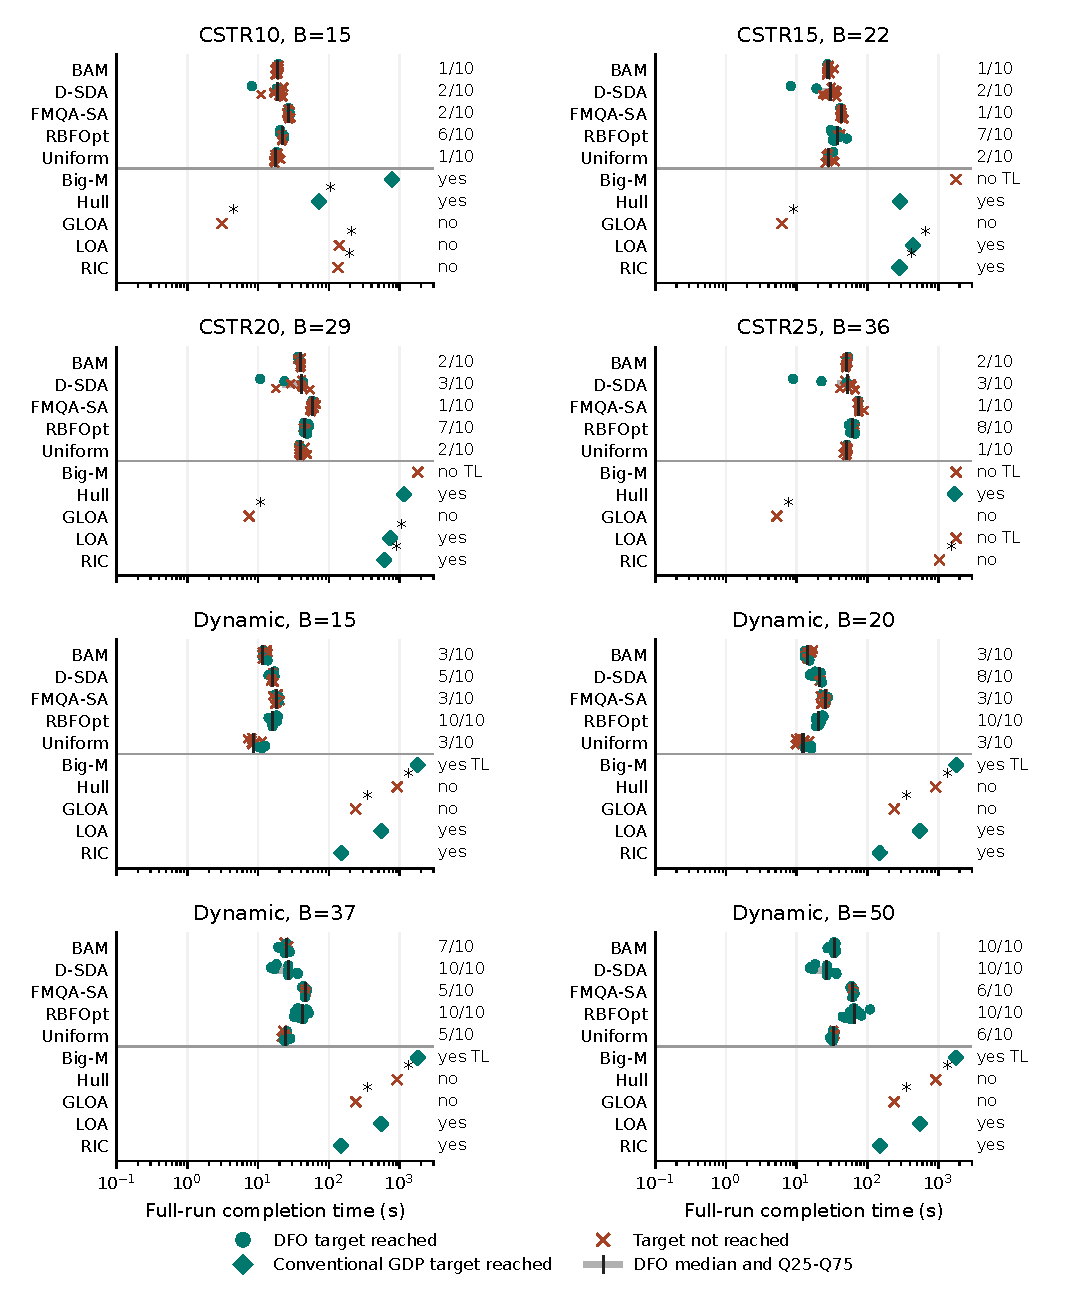
\includegraphics[width=\linewidth]{figures/joint_remaining_completion.pdf}
\caption{Joint full-run completion-time comparison for the eight additional process conditions.
Dots show successful DFO seeds, diamonds successful single conventional runs, and crosses target misses.
Gray segments and ticks show Q25--Q75 and medians across all ten DFO seeds.
TL denotes time-limit termination; asterisks mark bound inconsistencies (Section~\ref{sec:bound-audit}).
The Dynamic panels reuse the same conventional observations.
}
\label{fig:joint-remaining-completion}
\end{figure}
\FloatBarrier


\ifdefined\manuscriptwithsupplement
\FloatBarrier % \clearpage
\endgroup
\let\finishsupplement\relax
\else
\bibliographystyle{elsarticle-harv}
\bibliography{reference}
\def\finishsupplement{\end{document}}
\fi
\finishsupplement

\end{document}
